% Options for packages loaded elsewhere
% Options for packages loaded elsewhere
\PassOptionsToPackage{unicode}{hyperref}
\PassOptionsToPackage{hyphens}{url}
\PassOptionsToPackage{dvipsnames,svgnames,x11names}{xcolor}
%
\documentclass[
  11pt,
  letterpaper,
  DIV=11,
  numbers=noendperiod]{scrartcl}
\usepackage{xcolor}
\usepackage[left=25mm right=25mm top=25mm bottom=25mm]{geometry}
\usepackage{amsmath,amssymb}
\setcounter{secnumdepth}{5}
\usepackage{iftex}
\ifPDFTeX
  \usepackage[T1]{fontenc}
  \usepackage[utf8]{inputenc}
  \usepackage{textcomp} % provide euro and other symbols
\else % if luatex or xetex
  \usepackage{unicode-math} % this also loads fontspec
  \defaultfontfeatures{Scale=MatchLowercase}
  \defaultfontfeatures[\rmfamily]{Ligatures=TeX,Scale=1}
\fi
\usepackage{lmodern}
\ifPDFTeX\else
  % xetex/luatex font selection
  \setmainfont[]{Calibri}
  \setsansfont[]{Calibri}
  \setmonofont[]{Consolas}
\fi
% Use upquote if available, for straight quotes in verbatim environments
\IfFileExists{upquote.sty}{\usepackage{upquote}}{}
\IfFileExists{microtype.sty}{% use microtype if available
  \usepackage[]{microtype}
  \UseMicrotypeSet[protrusion]{basicmath} % disable protrusion for tt fonts
}{}
\makeatletter
\@ifundefined{KOMAClassName}{% if non-KOMA class
  \IfFileExists{parskip.sty}{%
    \usepackage{parskip}
  }{% else
    \setlength{\parindent}{0pt}
    \setlength{\parskip}{6pt plus 2pt minus 1pt}}
}{% if KOMA class
  \KOMAoptions{parskip=half}}
\makeatother
% Make \paragraph and \subparagraph free-standing
\makeatletter
\ifx\paragraph\undefined\else
  \let\oldparagraph\paragraph
  \renewcommand{\paragraph}{
    \@ifstar
      \xxxParagraphStar
      \xxxParagraphNoStar
  }
  \newcommand{\xxxParagraphStar}[1]{\oldparagraph*{#1}\mbox{}}
  \newcommand{\xxxParagraphNoStar}[1]{\oldparagraph{#1}\mbox{}}
\fi
\ifx\subparagraph\undefined\else
  \let\oldsubparagraph\subparagraph
  \renewcommand{\subparagraph}{
    \@ifstar
      \xxxSubParagraphStar
      \xxxSubParagraphNoStar
  }
  \newcommand{\xxxSubParagraphStar}[1]{\oldsubparagraph*{#1}\mbox{}}
  \newcommand{\xxxSubParagraphNoStar}[1]{\oldsubparagraph{#1}\mbox{}}
\fi
\makeatother

\usepackage{color}
\usepackage{fancyvrb}
\newcommand{\VerbBar}{|}
\newcommand{\VERB}{\Verb[commandchars=\\\{\}]}
\DefineVerbatimEnvironment{Highlighting}{Verbatim}{commandchars=\\\{\}}
% Add ',fontsize=\small' for more characters per line
\newenvironment{Shaded}{}{}
\newcommand{\AlertTok}[1]{\textcolor[rgb]{1.00,0.33,0.33}{\textbf{#1}}}
\newcommand{\AnnotationTok}[1]{\textcolor[rgb]{0.42,0.45,0.49}{#1}}
\newcommand{\AttributeTok}[1]{\textcolor[rgb]{0.84,0.23,0.29}{#1}}
\newcommand{\BaseNTok}[1]{\textcolor[rgb]{0.00,0.36,0.77}{#1}}
\newcommand{\BuiltInTok}[1]{\textcolor[rgb]{0.84,0.23,0.29}{#1}}
\newcommand{\CharTok}[1]{\textcolor[rgb]{0.01,0.18,0.38}{#1}}
\newcommand{\CommentTok}[1]{\textcolor[rgb]{0.42,0.45,0.49}{#1}}
\newcommand{\CommentVarTok}[1]{\textcolor[rgb]{0.42,0.45,0.49}{#1}}
\newcommand{\ConstantTok}[1]{\textcolor[rgb]{0.00,0.36,0.77}{#1}}
\newcommand{\ControlFlowTok}[1]{\textcolor[rgb]{0.84,0.23,0.29}{#1}}
\newcommand{\DataTypeTok}[1]{\textcolor[rgb]{0.84,0.23,0.29}{#1}}
\newcommand{\DecValTok}[1]{\textcolor[rgb]{0.00,0.36,0.77}{#1}}
\newcommand{\DocumentationTok}[1]{\textcolor[rgb]{0.42,0.45,0.49}{#1}}
\newcommand{\ErrorTok}[1]{\textcolor[rgb]{1.00,0.33,0.33}{\underline{#1}}}
\newcommand{\ExtensionTok}[1]{\textcolor[rgb]{0.84,0.23,0.29}{\textbf{#1}}}
\newcommand{\FloatTok}[1]{\textcolor[rgb]{0.00,0.36,0.77}{#1}}
\newcommand{\FunctionTok}[1]{\textcolor[rgb]{0.44,0.26,0.76}{#1}}
\newcommand{\ImportTok}[1]{\textcolor[rgb]{0.01,0.18,0.38}{#1}}
\newcommand{\InformationTok}[1]{\textcolor[rgb]{0.42,0.45,0.49}{#1}}
\newcommand{\KeywordTok}[1]{\textcolor[rgb]{0.84,0.23,0.29}{#1}}
\newcommand{\NormalTok}[1]{\textcolor[rgb]{0.14,0.16,0.18}{#1}}
\newcommand{\OperatorTok}[1]{\textcolor[rgb]{0.14,0.16,0.18}{#1}}
\newcommand{\OtherTok}[1]{\textcolor[rgb]{0.44,0.26,0.76}{#1}}
\newcommand{\PreprocessorTok}[1]{\textcolor[rgb]{0.84,0.23,0.29}{#1}}
\newcommand{\RegionMarkerTok}[1]{\textcolor[rgb]{0.42,0.45,0.49}{#1}}
\newcommand{\SpecialCharTok}[1]{\textcolor[rgb]{0.00,0.36,0.77}{#1}}
\newcommand{\SpecialStringTok}[1]{\textcolor[rgb]{0.01,0.18,0.38}{#1}}
\newcommand{\StringTok}[1]{\textcolor[rgb]{0.01,0.18,0.38}{#1}}
\newcommand{\VariableTok}[1]{\textcolor[rgb]{0.89,0.38,0.04}{#1}}
\newcommand{\VerbatimStringTok}[1]{\textcolor[rgb]{0.01,0.18,0.38}{#1}}
\newcommand{\WarningTok}[1]{\textcolor[rgb]{1.00,0.33,0.33}{#1}}

\usepackage{longtable,booktabs,array}
\newcounter{none} % for unnumbered tables
\usepackage{calc} % for calculating minipage widths
% Correct order of tables after \paragraph or \subparagraph
\usepackage{etoolbox}
\makeatletter
\patchcmd\longtable{\par}{\if@noskipsec\mbox{}\fi\par}{}{}
\makeatother
% Allow footnotes in longtable head/foot
\IfFileExists{footnotehyper.sty}{\usepackage{footnotehyper}}{\usepackage{footnote}}
\makesavenoteenv{longtable}
\usepackage{graphicx}
\makeatletter
\newsavebox\pandoc@box
\newcommand*\pandocbounded[1]{% scales image to fit in text height/width
  \sbox\pandoc@box{#1}%
  \Gscale@div\@tempa{\textheight}{\dimexpr\ht\pandoc@box+\dp\pandoc@box\relax}%
  \Gscale@div\@tempb{\linewidth}{\wd\pandoc@box}%
  \ifdim\@tempb\p@<\@tempa\p@\let\@tempa\@tempb\fi% select the smaller of both
  \ifdim\@tempa\p@<\p@\scalebox{\@tempa}{\usebox\pandoc@box}%
  \else\usebox{\pandoc@box}%
  \fi%
}
% Set default figure placement to htbp
\def\fps@figure{htbp}
\makeatother





\setlength{\emergencystretch}{3em} % prevent overfull lines

\providecommand{\tightlist}{%
  \setlength{\itemsep}{0pt}\setlength{\parskip}{0pt}}



 


\usepackage{lastpage}
\usepackage{scrlayer-scrpage}
\lofoot{STRADA81}
\cfoot{\thepage/\pageref{LastPage}}
\rofoot{Confidential}
\KOMAoption{captions}{tableheading}
\makeatletter
\@ifpackageloaded{caption}{}{\usepackage{caption}}
\AtBeginDocument{%
\ifdefined\contentsname
  \renewcommand*\contentsname{Table of contents}
\else
  \newcommand\contentsname{Table of contents}
\fi
\ifdefined\listfigurename
  \renewcommand*\listfigurename{List of Figures}
\else
  \newcommand\listfigurename{List of Figures}
\fi
\ifdefined\listtablename
  \renewcommand*\listtablename{List of Tables}
\else
  \newcommand\listtablename{List of Tables}
\fi
\ifdefined\figurename
  \renewcommand*\figurename{Figure}
\else
  \newcommand\figurename{Figure}
\fi
\ifdefined\tablename
  \renewcommand*\tablename{Table}
\else
  \newcommand\tablename{Table}
\fi
}
\@ifpackageloaded{float}{}{\usepackage{float}}
\floatstyle{ruled}
\@ifundefined{c@chapter}{\newfloat{codelisting}{h}{lop}}{\newfloat{codelisting}{h}{lop}[chapter]}
\floatname{codelisting}{Listing}
\newcommand*\listoflistings{\listof{codelisting}{List of Listings}}
\makeatother
\makeatletter
\makeatother
\makeatletter
\@ifpackageloaded{caption}{}{\usepackage{caption}}
\@ifpackageloaded{subcaption}{}{\usepackage{subcaption}}
\makeatother
\usepackage{bookmark}
\IfFileExists{xurl.sty}{\usepackage{xurl}}{} % add URL line breaks if available
\urlstyle{same}
% fallback for those not using the hyperref driver hyperxmp:
\makeatletter
\@ifundefined{xmpquote}{\newcommand{\xmpquote}[1]{#1}}{}
\makeatother
\hypersetup{
  pdftitle={Test Execution Logging Design},
  pdfauthor={Nenad Samardzic},
  colorlinks=true,
  linkcolor={blue},
  filecolor={Maroon},
  citecolor={Blue},
  urlcolor={Blue},
  pdfcreator={LaTeX via pandoc}}


\title{Test Execution Logging Design}
\author{Nenad Samardzic}
\date{2026-09-25}
\begin{document}
\maketitle

\renewcommand*\contentsname{Table of contents}
{
\setcounter{tocdepth}{3}
\tableofcontents
}

\section{Purpose}\label{purpose}

This document defines the architecture, format, collection, storage,
processing, analysis, and lifecycle of test execution logs generated
during System-on-Chip (SoC) validation.

The objectives are:

\begin{itemize}
\tightlist
\item
  complete traceability of every test execution;
\item
  a consistent logging mechanism across different test types;
\item
  correlation between test actions and SoC responses;
\item
  preservation of raw diagnostic information;
\item
  machine-readable data for automated analysis;
\item
  human-readable logs for debugging;
\item
  integration with Continuous Integration and Continuous Delivery
  (CI/CD) and test reports;
\item
  reproducibility of failures;
\item
  long-term historical analysis and regression detection.
\end{itemize}

The logging system supports both \textbf{interactive/local execution}
and \textbf{automated CI execution}.

\section{Scope}\label{scope}

The logging architecture covers the complete execution chain.

\begin{figure}

\centering{

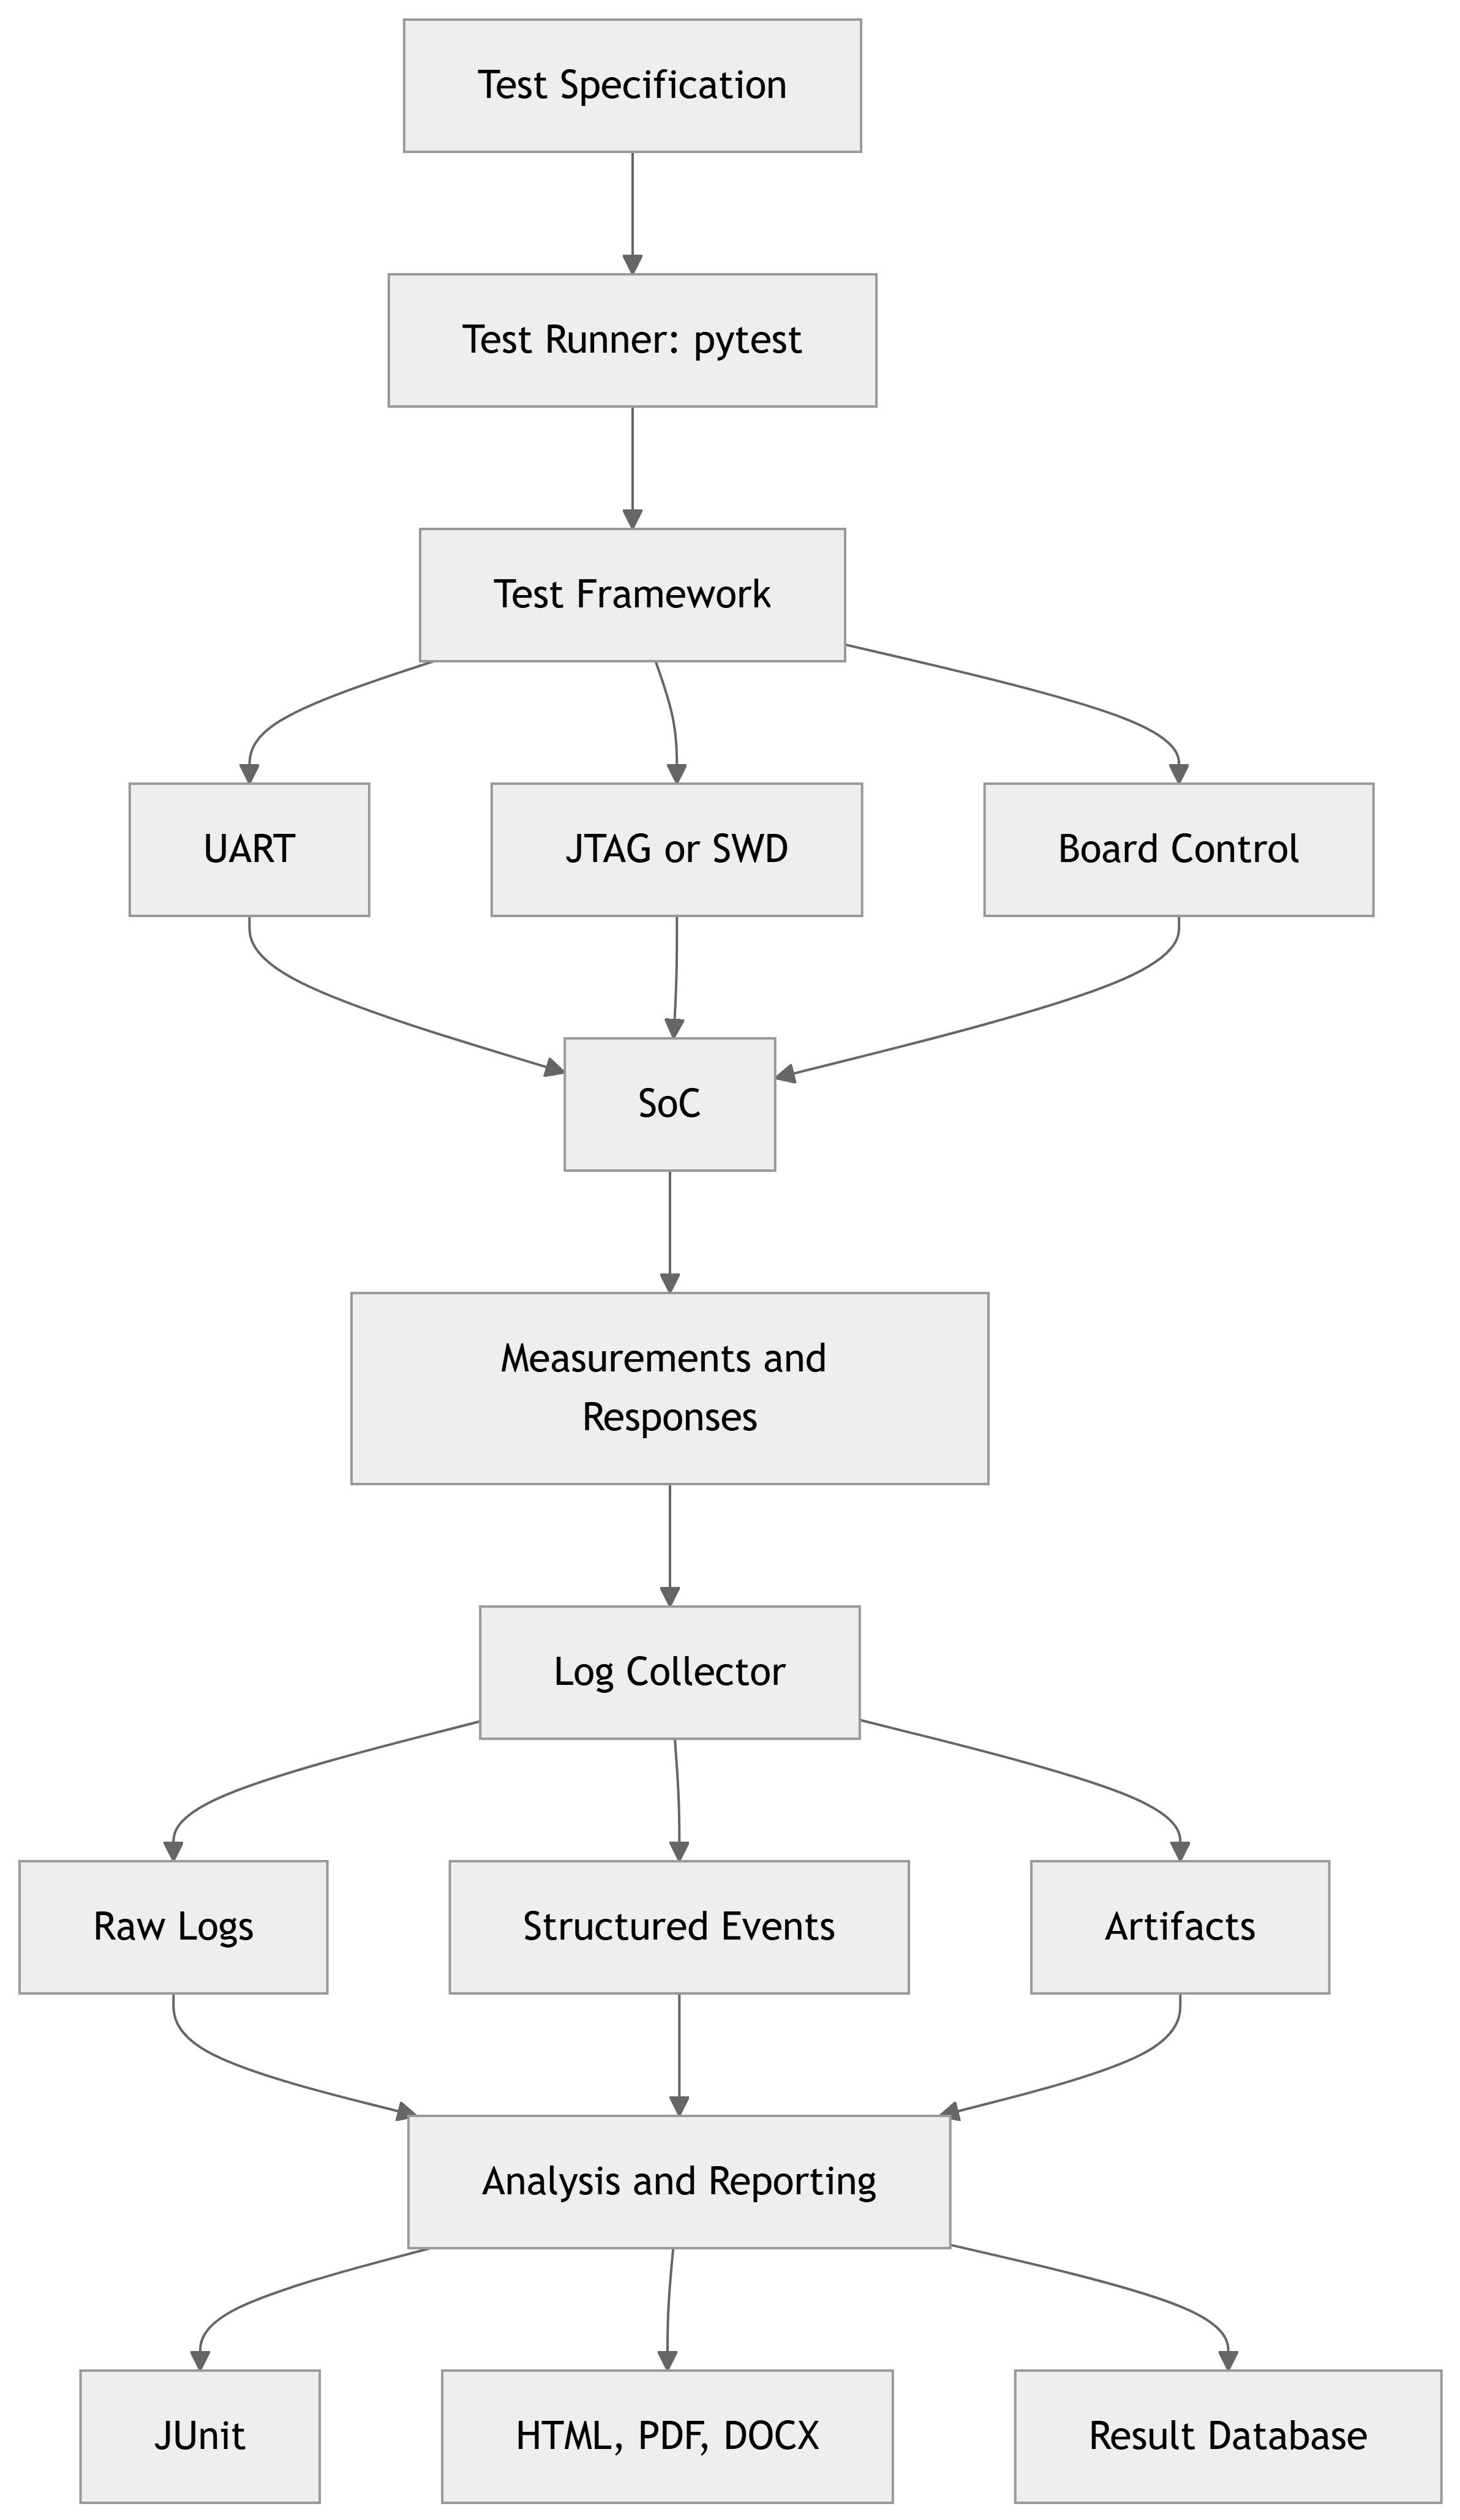
\includegraphics[width=6.21in,height=10.73in]{gtp_logging_v2_files/figure-latex/mermaid-figure-1.png}

}

\caption{\label{fig-execution-chain}Complete SoC validation execution
and logging chain}

\end{figure}%

\section{Design Goals}\label{design-goals}

These goals are explicit requirements.

\subsection{Functional Requirements}\label{functional-requirements}

{\def\LTcaptype{none} % do not increment counter
\begin{longtable}[]{@{}ll@{}}
\toprule\noalign{}
ID & Requirement \\
\midrule\noalign{}
\endhead
\bottomrule\noalign{}
\endlastfoot
LOG-001 & Every test execution shall have a unique Execution ID. \\
LOG-002 & Every test case shall have a unique Test ID. \\
LOG-003 & All log entries shall be associated with an Execution ID. \\
LOG-004 & Logs from different interfaces shall be correlatable. \\
LOG-005 & Raw interface output shall be preserved. \\
LOG-006 & Log entries shall contain timestamps. \\
LOG-007 & Test actions shall be logged. \\
LOG-008 & Test verdicts shall be logged. \\
LOG-009 & Failures shall contain sufficient diagnostic information. \\
LOG-010 & Logs shall be machine-readable. \\
LOG-011 & Logs shall be human-readable. \\
LOG-012 & Logs shall be usable outside the CI environment. \\
LOG-013 & Test artifacts shall be associated with the execution. \\
LOG-014 & Logging shall have minimal impact on test execution. \\
LOG-015 & Logs shall support long-term historical analysis. \\
\end{longtable}
}

\section{Logging Architecture}\label{logging-architecture}

The logging system is separated into four logical layers.

\begin{figure}

\centering{

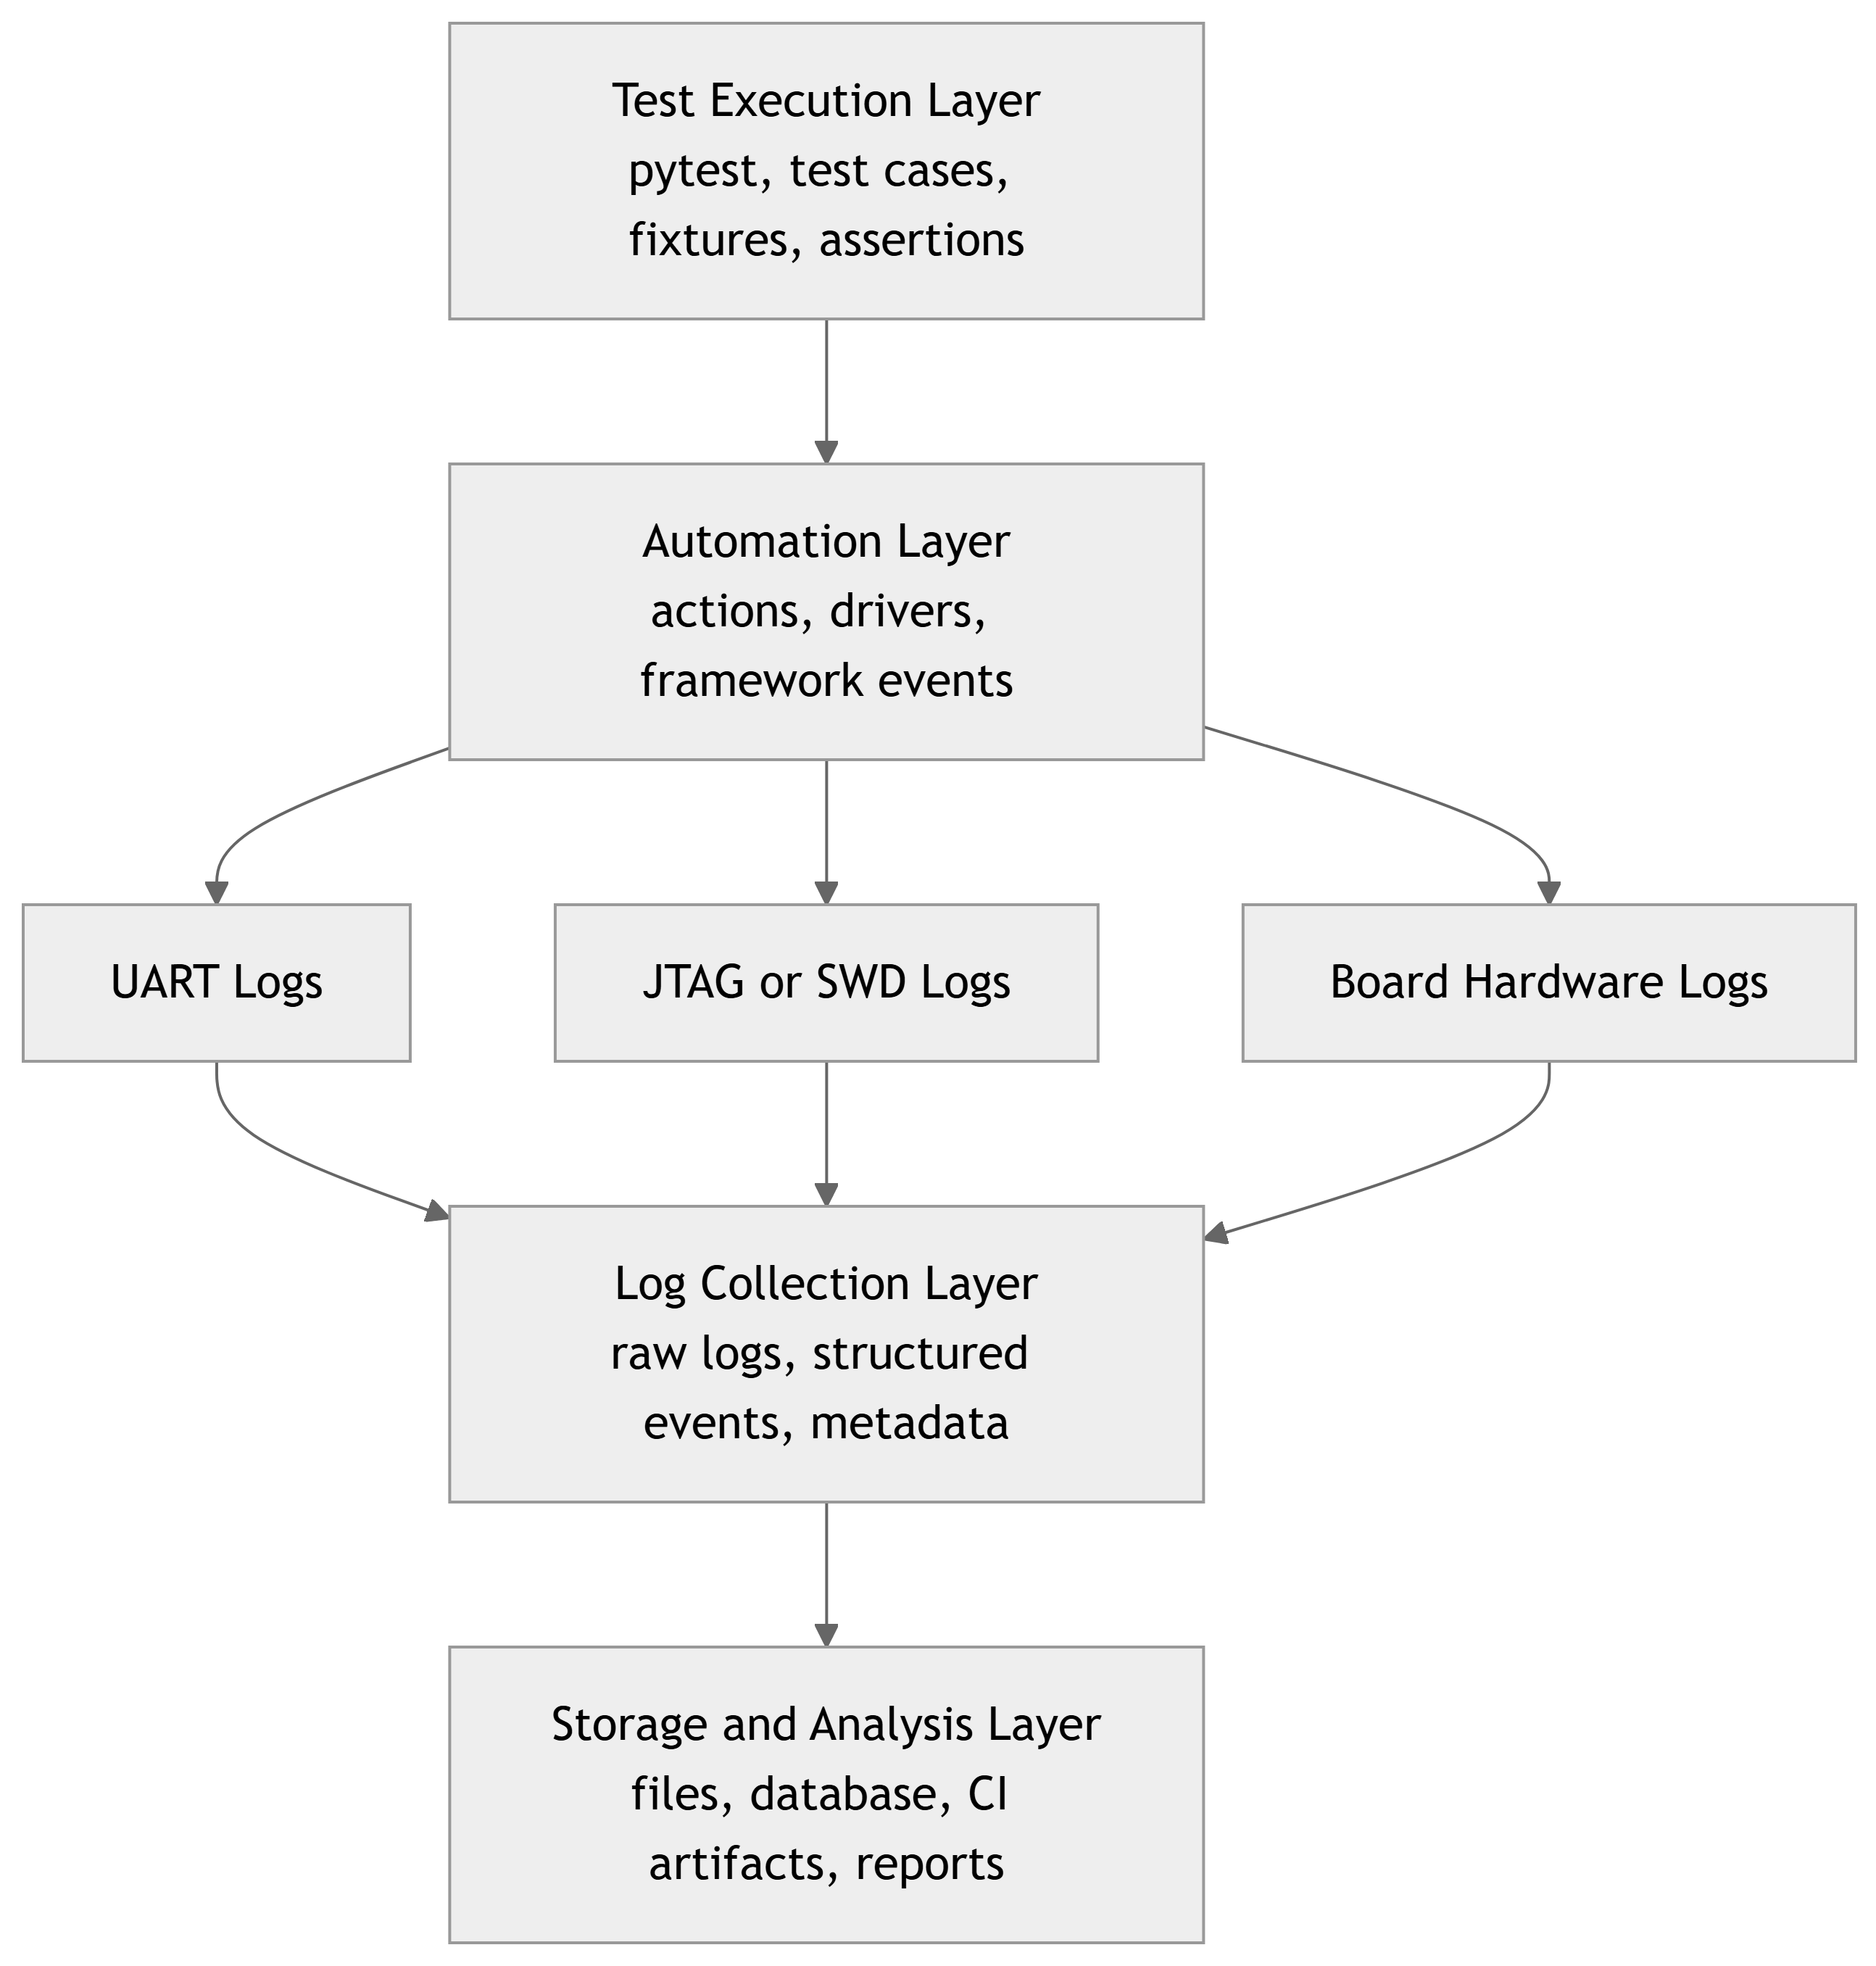
\includegraphics[width=6.75in,height=7.06in]{gtp_logging_v2_files/figure-latex/mermaid-figure-13.png}

}

\caption{\label{fig-logging-layers}Logical logging architecture}

\end{figure}%

This separation is important because \textbf{raw logs and interpreted
logs are different data products}.

\section{What Should Be Logged?}\label{what-should-be-logged}

Logs are divided into well-defined categories.

\subsection{Test Framework Logs}\label{test-framework-logs}

Generated by pytest or the test framework. Typical events are:

\begin{verbatim}
TEST_START
TEST_STEP
TEST_PASS
TEST_FAIL
TEST_SKIP
TEST_ERROR
TEST_END
\end{verbatim}

Example:

\begin{verbatim}
10:21:15.120 INFO  TEST_START
10:21:15.124 INFO  test_id=SOC_UART_001
10:21:15.125 INFO  step="Reset DUT"
10:21:17.342 INFO  step="Wait for boot"
10:21:18.002 INFO  step="Send UART command"
10:21:18.103 INFO  step="Validate response"
10:21:18.104 INFO  TEST_PASS
\end{verbatim}

\subsection{Test Action Logs}\label{test-action-logs}

Every significant action performed by the automation framework is
logged, including power control, reset, firmware flashing, interface
operations, register access, measurements, and debugger operations.

\begin{verbatim}
ACTION
execution_id=EXE-20260918-001
test_id=SOC_UART_001
action=UART_SEND
interface=UART0
data="AT+STATUS"
\end{verbatim}

\subsection{SoC Interface Logs}\label{soc-interface-logs}

\subsubsection{UART}\label{uart}

Recommended fields are \texttt{timestamp}, \texttt{interface},
\texttt{direction}, \texttt{data}, and \texttt{baudrate}.

\begin{verbatim}
12:31:02.120 UART0 TX  "status\r\n"
12:31:02.145 UART0 RX  "STATUS: READY\r\n"
\end{verbatim}

\subsubsection{SPI}\label{spi}

\begin{verbatim}
SPI0
TX: 9F 00 00 00
RX: EF 40 18 00
\end{verbatim}

\subsubsection{I2C}\label{i2c}

\begin{verbatim}
I2C0
ADDR=0x50
WRITE=00 10
READ=AB CD
\end{verbatim}

\subsubsection{JTAG/SWD}\label{jtagswd}

Typical events include connect, reset, halt, resume, register read,
memory read, and memory write.

\subsection{Firmware Logs}\label{firmware-logs}

Firmware-generated messages are preserved separately from automation
logs.

\begin{verbatim}
[BOOT] Starting system
[CLK] PLL configured
[MEM] DDR initialization OK
[UART] Driver initialized
[APP] Application started
\end{verbatim}

The source remains explicit:

\begin{verbatim}
source = DUT
interface = UART0
\end{verbatim}

Do not merge firmware output into the Python log and discard its origin.

\subsection{Hardware and Board Logs}\label{hardware-and-board-logs}

Capture the power-supply state, voltage, current, temperature, reset
state, relay state, board-controller messages, power-cycle events, and
external instrumentation.

\begin{verbatim}
BOARD_POWER_ON
voltage=3.30V
current=142mA
timestamp=2026-09-18T12:31:00.123Z
\end{verbatim}

\subsection{Environment Information}\label{environment-information}

Every execution captures the environment in which the test was executed.

\begin{Shaded}
\begin{Highlighting}[]
\FunctionTok{execution}\KeywordTok{:}
\AttributeTok{  }\FunctionTok{execution\_id}\KeywordTok{:}\AttributeTok{ EXE{-}20260918{-}001}
\AttributeTok{  }\FunctionTok{timestamp}\KeywordTok{:}\AttributeTok{ 2026{-}09{-}18T12:30:00Z}
\FunctionTok{test}\KeywordTok{:}
\AttributeTok{  }\FunctionTok{suite}\KeywordTok{:}\AttributeTok{ regression}
\AttributeTok{  }\FunctionTok{test\_id}\KeywordTok{:}\AttributeTok{ SOC\_UART\_001}
\AttributeTok{  }\FunctionTok{test\_version}\KeywordTok{:}\AttributeTok{ abc1234}
\FunctionTok{dut}\KeywordTok{:}
\AttributeTok{  }\FunctionTok{device}\KeywordTok{:}\AttributeTok{ XYZ123}
\AttributeTok{  }\FunctionTok{silicon\_revision}\KeywordTok{:}\AttributeTok{ B1}
\AttributeTok{  }\FunctionTok{serial\_number}\KeywordTok{:}\AttributeTok{ DUT{-}00017}
\AttributeTok{  }\FunctionTok{board\_revision}\KeywordTok{:}\AttributeTok{ REV\_C}
\FunctionTok{firmware}\KeywordTok{:}
\AttributeTok{  }\FunctionTok{version}\KeywordTok{:}\AttributeTok{ }\FloatTok{2.4.1}
\AttributeTok{  }\FunctionTok{git\_commit}\KeywordTok{:}\AttributeTok{ 8f23ab1}
\AttributeTok{  }\FunctionTok{build\_id}\KeywordTok{:}\AttributeTok{ BUILD{-}12345}
\FunctionTok{environment}\KeywordTok{:}
\AttributeTok{  }\FunctionTok{runner}\KeywordTok{:}\AttributeTok{ Jenkins}
\AttributeTok{  }\FunctionTok{runner\_id}\KeywordTok{:}\AttributeTok{ runner{-}04}
\AttributeTok{  }\FunctionTok{python\_version}\KeywordTok{:}\AttributeTok{ }\StringTok{"3.12"}
\AttributeTok{  }\FunctionTok{pytest\_version}\KeywordTok{:}\AttributeTok{ }\StringTok{"8.x"}
\AttributeTok{  }\FunctionTok{os}\KeywordTok{:}\AttributeTok{ Ubuntu 24.04}
\FunctionTok{tools}\KeywordTok{:}
\AttributeTok{  }\FunctionTok{debugger}\KeywordTok{:}\AttributeTok{ J{-}Link}
\AttributeTok{  }\FunctionTok{debugger\_version}\KeywordTok{:}\AttributeTok{ x.x.x}
\end{Highlighting}
\end{Shaded}

This information is critical for failure reproduction.

\section{Identification and
Correlation}\label{identification-and-correlation}

\subsection{Execution ID}\label{execution-id}

The \textbf{Execution ID} is the primary correlation mechanism. Example:

\begin{verbatim}
EXE-20260918-153045-7F32
\end{verbatim}

Everything generated during one run references the same Execution ID.

\begin{figure}

\centering{

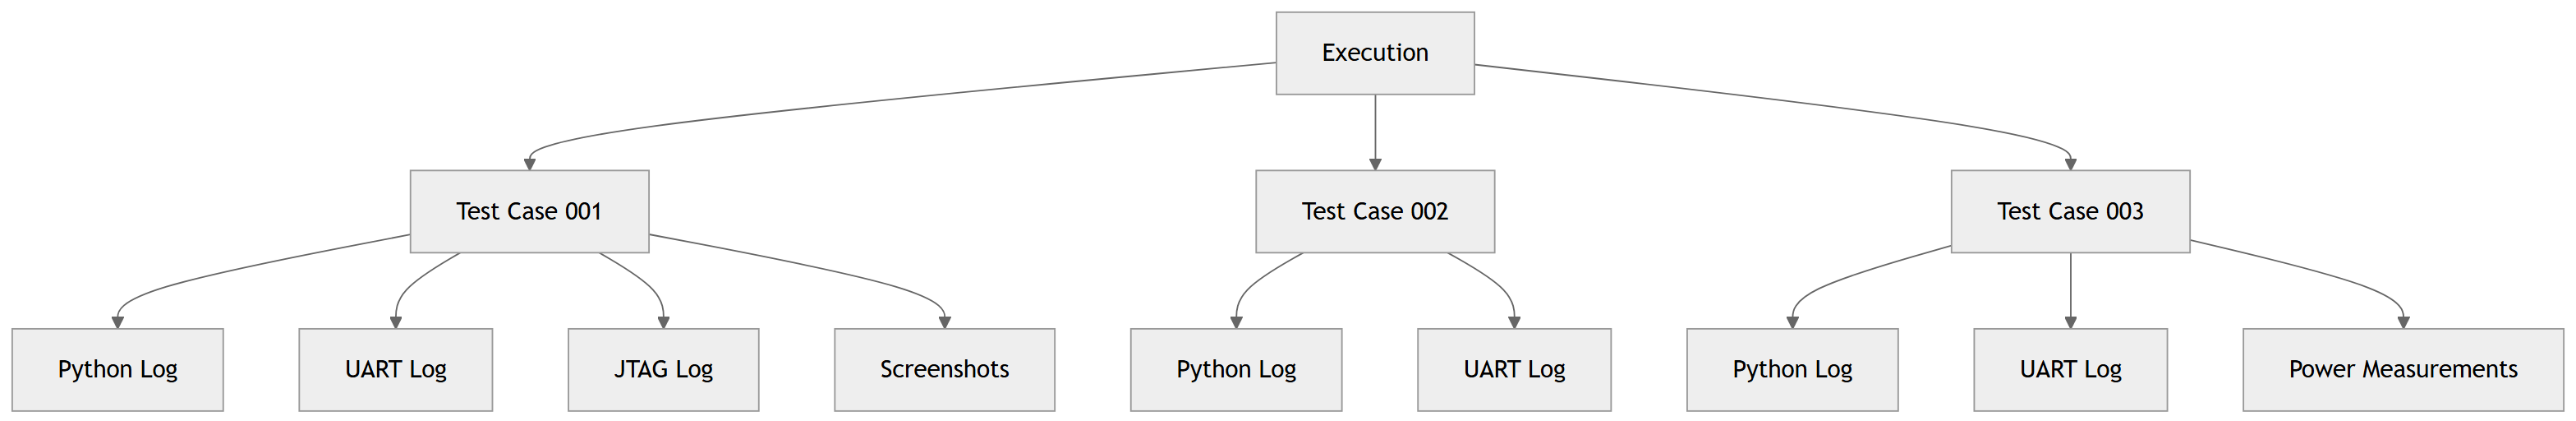
\includegraphics[width=17.64in,height=2.9in]{gtp_logging_v2_files/figure-latex/mermaid-figure-12.png}

}

\caption{\label{fig-execution-tree}Execution-level artifact hierarchy}

\end{figure}%

\subsection{Test ID}\label{test-id}

Each test has a stable identifier, for example:

\begin{verbatim}
SOC-BOOT-001
SOC-UART-001
SOC-SPI-014
SOC-INT-023
SOC-PWR-007
\end{verbatim}

Do not use only the Python function name. Associate a stable logical ID
with the test:

\begin{Shaded}
\begin{Highlighting}[]
\AttributeTok{@pytest.mark.test\_id}\NormalTok{(}\StringTok{"SOC{-}UART{-}001"}\NormalTok{)}
\KeywordTok{def}\NormalTok{ test\_uart\_command():}
\NormalTok{    ...}
\end{Highlighting}
\end{Shaded}

\subsection{Step ID}\label{step-id}

Complex tests use explicit step identifiers.

\begin{verbatim}
TEST: SOC-UART-001
STEP-001  Power on DUT
STEP-002  Flash firmware
STEP-003  Reset DUT
STEP-004  Wait for boot
STEP-005  Send command
STEP-006  Validate response
STEP-007  Power off DUT
\end{verbatim}

A precise failure record is:

\begin{verbatim}
test_id=SOC-UART-001
step_id=STEP-005
status=FAILED
\end{verbatim}

\subsection{Correlation ID}\label{correlation-id}

For complex operations, use an additional \texttt{correlation\_id} to
group low-level events that belong to one high-level action.

\begin{figure}

\centering{

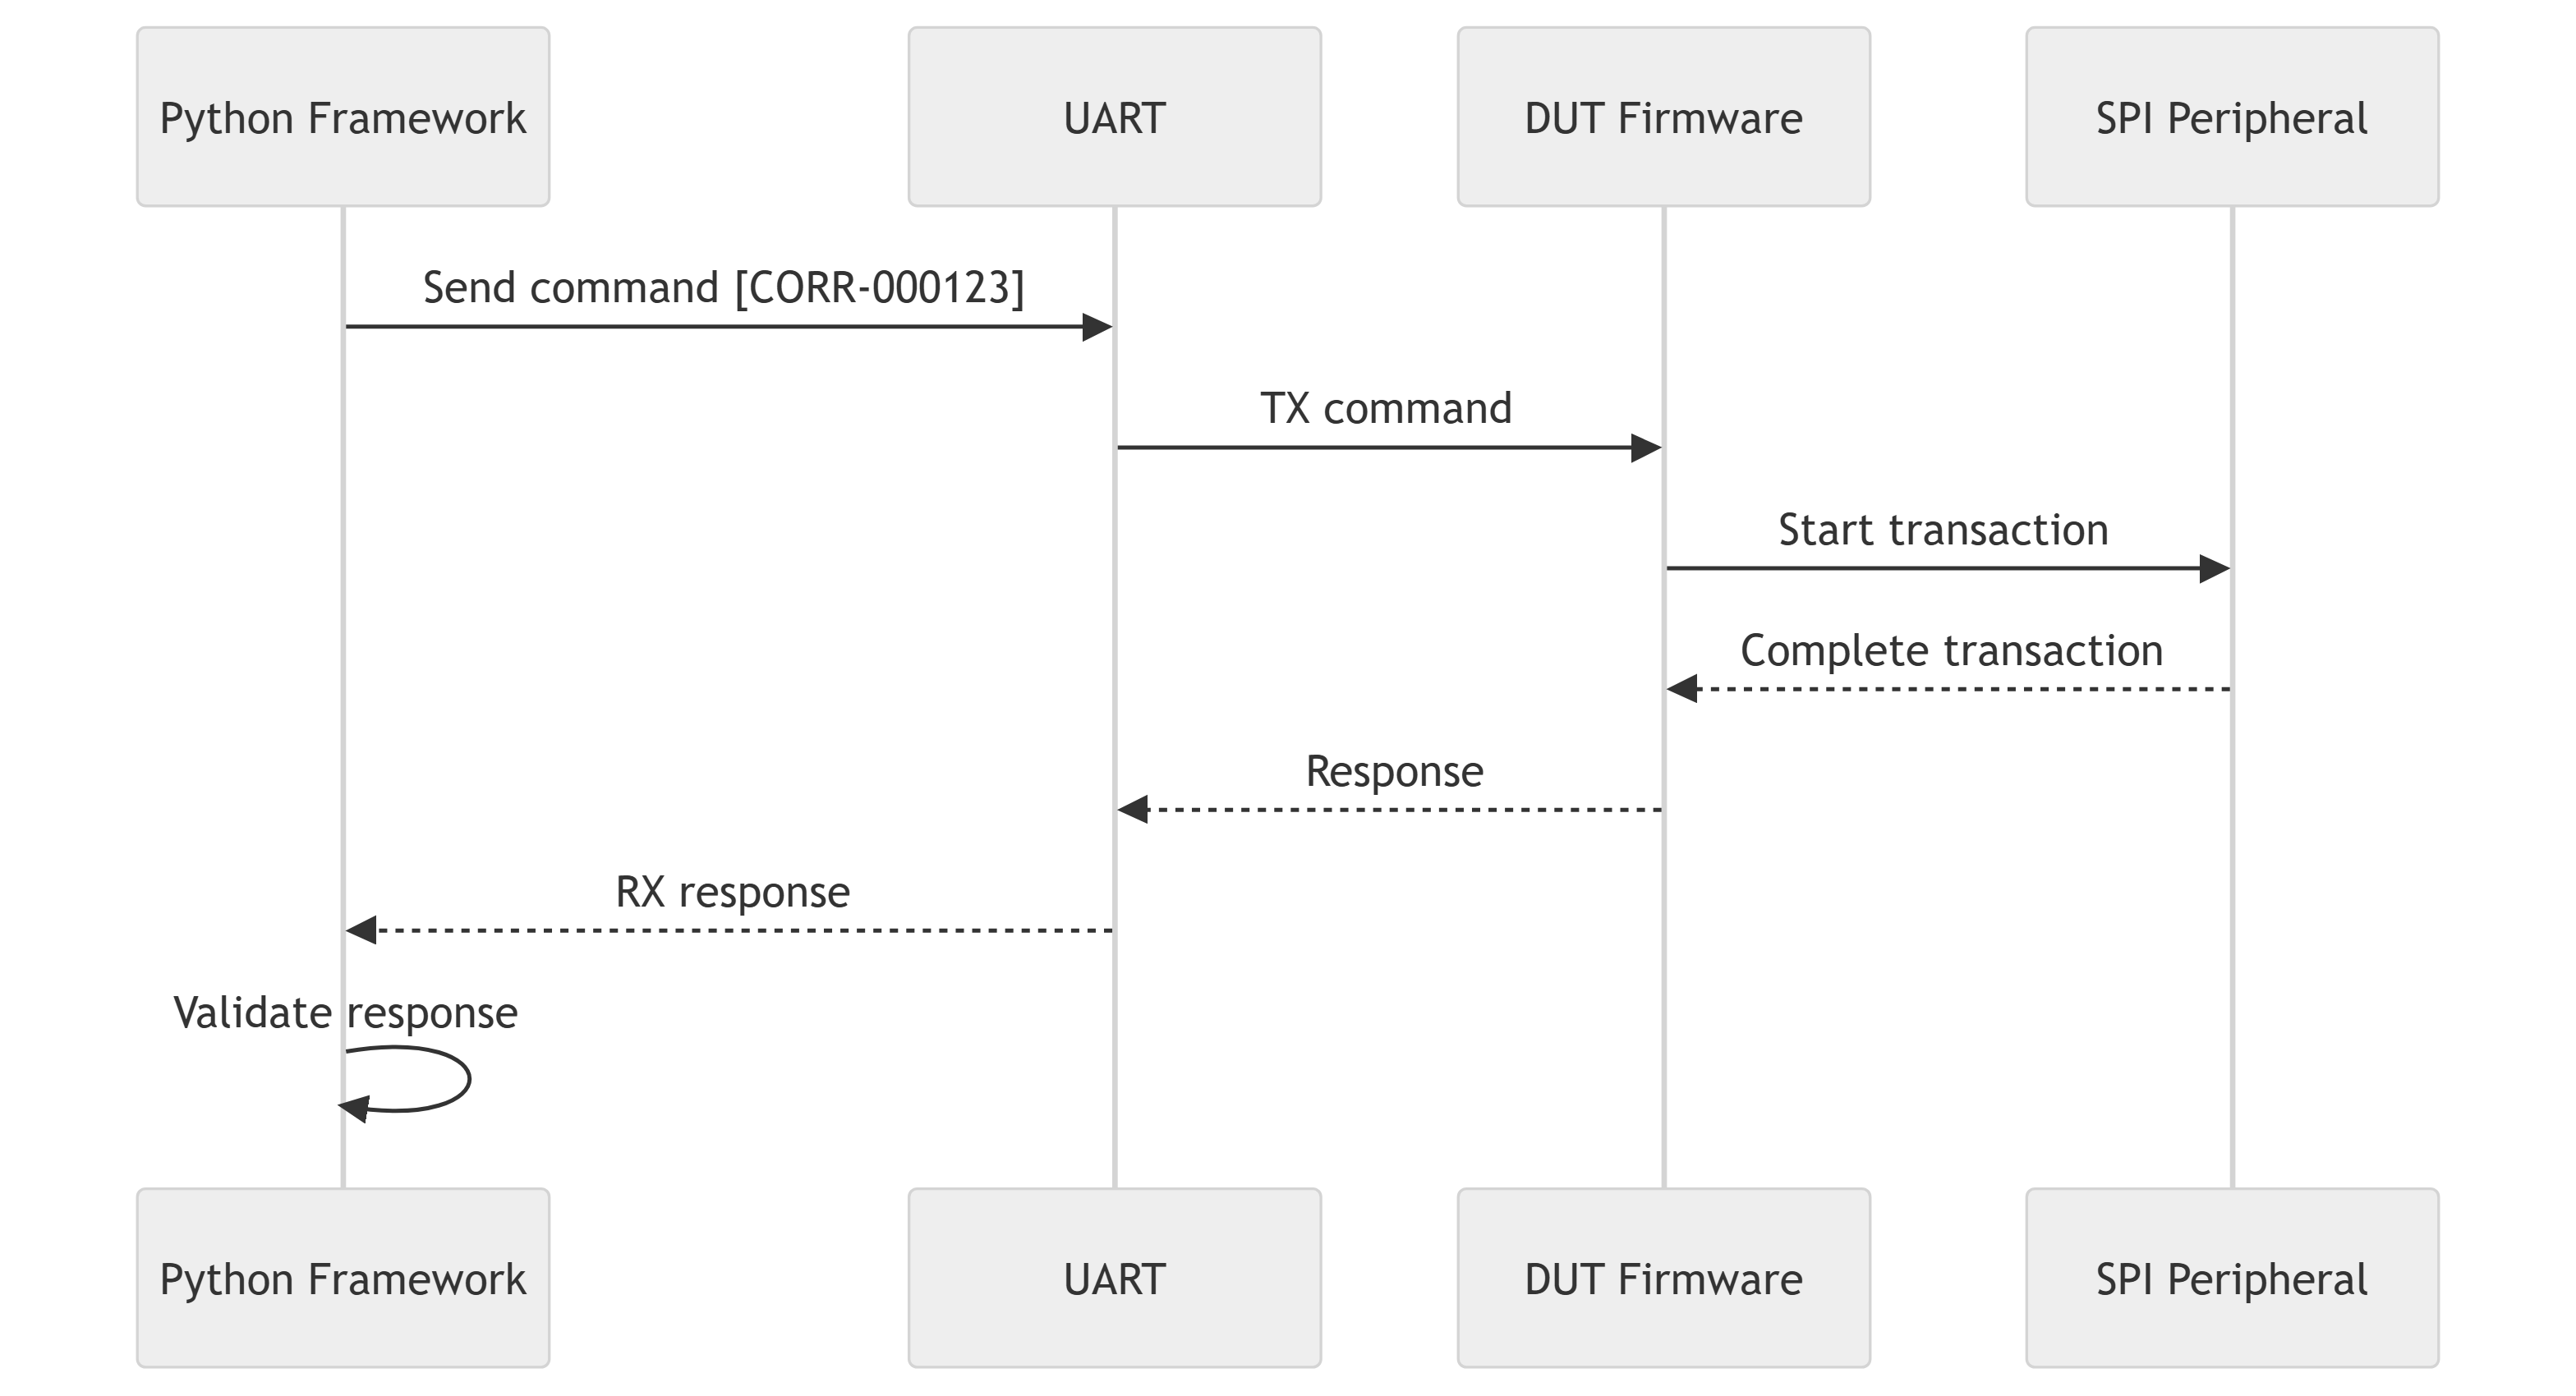
\includegraphics[width=9.77in,height=5.3in]{gtp_logging_v2_files/figure-latex/mermaid-figure-11.png}

}

\caption{\label{fig-correlation}Correlation of one high-level operation
across log sources}

\end{figure}%

\section{Log Entry Structure}\label{log-entry-structure}

The canonical machine-readable format is \textbf{JSON Lines (JSONL)}.
One event corresponds to one JSON object.

\begin{Shaded}
\begin{Highlighting}[]
\FunctionTok{\{}
    \DataTypeTok{"timestamp"}\FunctionTok{:} \StringTok{"2026{-}09{-}18T12:31:02.120Z"}\FunctionTok{,}
    \DataTypeTok{"execution\_id"}\FunctionTok{:} \StringTok{"EXE{-}20260918{-}001"}\FunctionTok{,}
    \DataTypeTok{"test\_id"}\FunctionTok{:} \StringTok{"SOC{-}UART{-}001"}\FunctionTok{,}
    \DataTypeTok{"source"}\FunctionTok{:} \StringTok{"test\_framework"}\FunctionTok{,}
    \DataTypeTok{"level"}\FunctionTok{:} \StringTok{"INFO"}\FunctionTok{,}
    \DataTypeTok{"event"}\FunctionTok{:} \StringTok{"TEST\_START"}\FunctionTok{,}
    \DataTypeTok{"message"}\FunctionTok{:} \StringTok{"UART test started"}
\FunctionTok{\}}
\end{Highlighting}
\end{Shaded}

\begin{Shaded}
\begin{Highlighting}[]
\FunctionTok{\{}
    \DataTypeTok{"timestamp"}\FunctionTok{:} \StringTok{"2026{-}09{-}18T12:31:05.120Z"}\FunctionTok{,}
    \DataTypeTok{"execution\_id"}\FunctionTok{:} \StringTok{"EXE{-}20260918{-}001"}\FunctionTok{,}
    \DataTypeTok{"test\_id"}\FunctionTok{:} \StringTok{"SOC{-}UART{-}001"}\FunctionTok{,}
    \DataTypeTok{"source"}\FunctionTok{:} \StringTok{"uart"}\FunctionTok{,}
    \DataTypeTok{"interface"}\FunctionTok{:} \StringTok{"UART0"}\FunctionTok{,}
    \DataTypeTok{"direction"}\FunctionTok{:} \StringTok{"TX"}\FunctionTok{,}
    \DataTypeTok{"event"}\FunctionTok{:} \StringTok{"DATA"}\FunctionTok{,}
    \DataTypeTok{"data"}\FunctionTok{:} \StringTok{"status}\CharTok{\textbackslash{}\textbackslash{}}\StringTok{r}\CharTok{\textbackslash{}\textbackslash{}}\StringTok{n"}
\FunctionTok{\}}
\end{Highlighting}
\end{Shaded}

\subsection{Recommended Event Schema}\label{recommended-event-schema}

Mandatory fields:

{\def\LTcaptype{none} % do not increment counter
\begin{longtable}[]{@{}ll@{}}
\toprule\noalign{}
Field & Description \\
\midrule\noalign{}
\endhead
\bottomrule\noalign{}
\endlastfoot
\texttt{timestamp} & Event timestamp in Coordinated Universal Time
(UTC). \\
\texttt{execution\_id} & Unique execution identifier. \\
\texttt{source} & Component that generated the event. \\
\texttt{level} & Event severity. \\
\texttt{event} & Event type. \\
\end{longtable}
}

Contextual fields:

{\def\LTcaptype{none} % do not increment counter
\begin{longtable}[]{@{}ll@{}}
\toprule\noalign{}
Field & Description \\
\midrule\noalign{}
\endhead
\bottomrule\noalign{}
\endlastfoot
\texttt{test\_id} & Test-case identifier. \\
\texttt{step\_id} & Test-step identifier. \\
\texttt{correlation\_id} & Operation correlation identifier. \\
\texttt{interface} & DUT interface. \\
\texttt{dut\_id} & DUT identifier. \\
\texttt{board\_id} & Board identifier. \\
\texttt{message} & Human-readable description. \\
\texttt{data} & Raw or structured event data. \\
\end{longtable}
}

\section{Log Levels}\label{log-levels}

{\def\LTcaptype{none} % do not increment counter
\begin{longtable}[]{@{}ll@{}}
\toprule\noalign{}
Level & Purpose \\
\midrule\noalign{}
\endhead
\bottomrule\noalign{}
\endlastfoot
TRACE & Extremely detailed diagnostic information. \\
DEBUG & Developer and debugging information. \\
INFO & Normal execution information. \\
WARNING & Unexpected but non-fatal condition. \\
ERROR & Test or framework error. \\
CRITICAL & Infrastructure or system failure. \\
\end{longtable}
}

\begin{verbatim}
INFO     Flashing firmware
INFO     Firmware flash completed
DEBUG    Waiting for boot message
INFO     DUT boot completed
WARNING  Boot took longer than expected
ERROR    UART response timeout
\end{verbatim}

\section{Raw and Processed Logs}\label{raw-and-processed-logs}

\begin{quote}
\textbf{Architectural rule:} Never destroy the raw evidence.
\end{quote}

\begin{figure}

\centering{

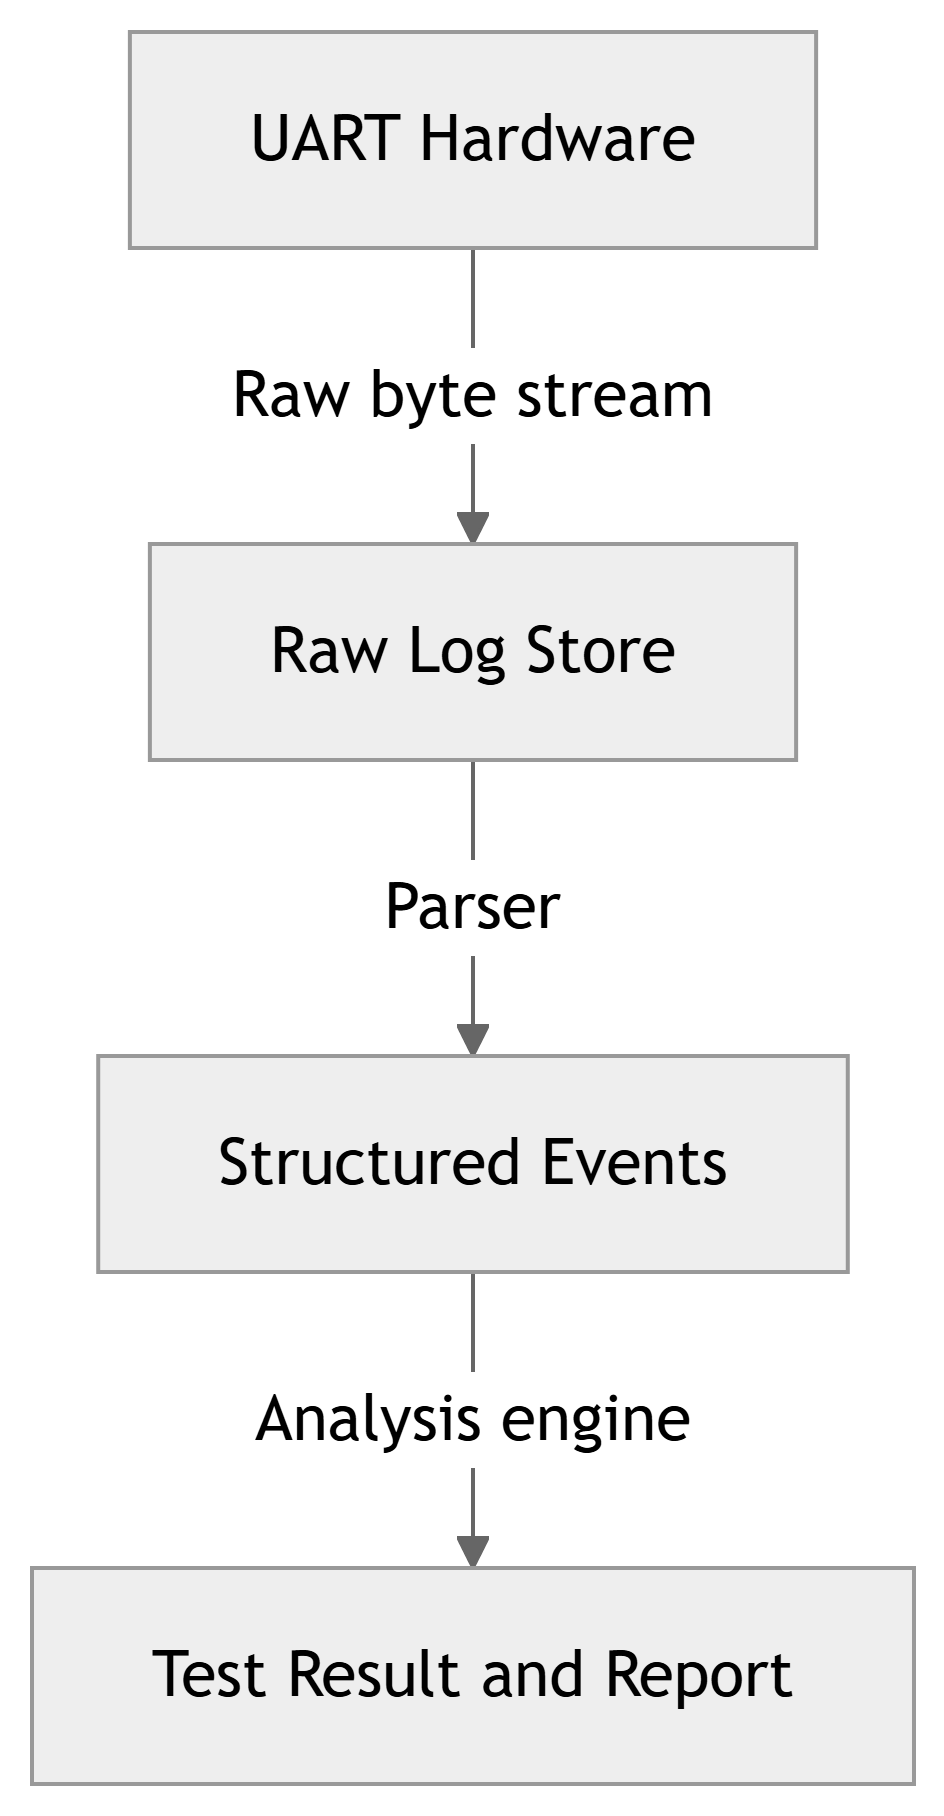
\includegraphics[width=2.46in,height=4.73in]{gtp_logging_v2_files/figure-latex/mermaid-figure-10.png}

}

\caption{\label{fig-raw-processed}Raw-to-processed logging flow}

\end{figure}%

If the parser has a defect, raw logs can be reprocessed. If only parsed
output is stored, the original evidence is lost.

\section{Storage Architecture}\label{storage-architecture}

For the initial implementation, a filesystem-based artifact structure is
sufficient. A centralized logging platform is introduced only when log
volume and search requirements justify it.

\begin{figure}

\centering{

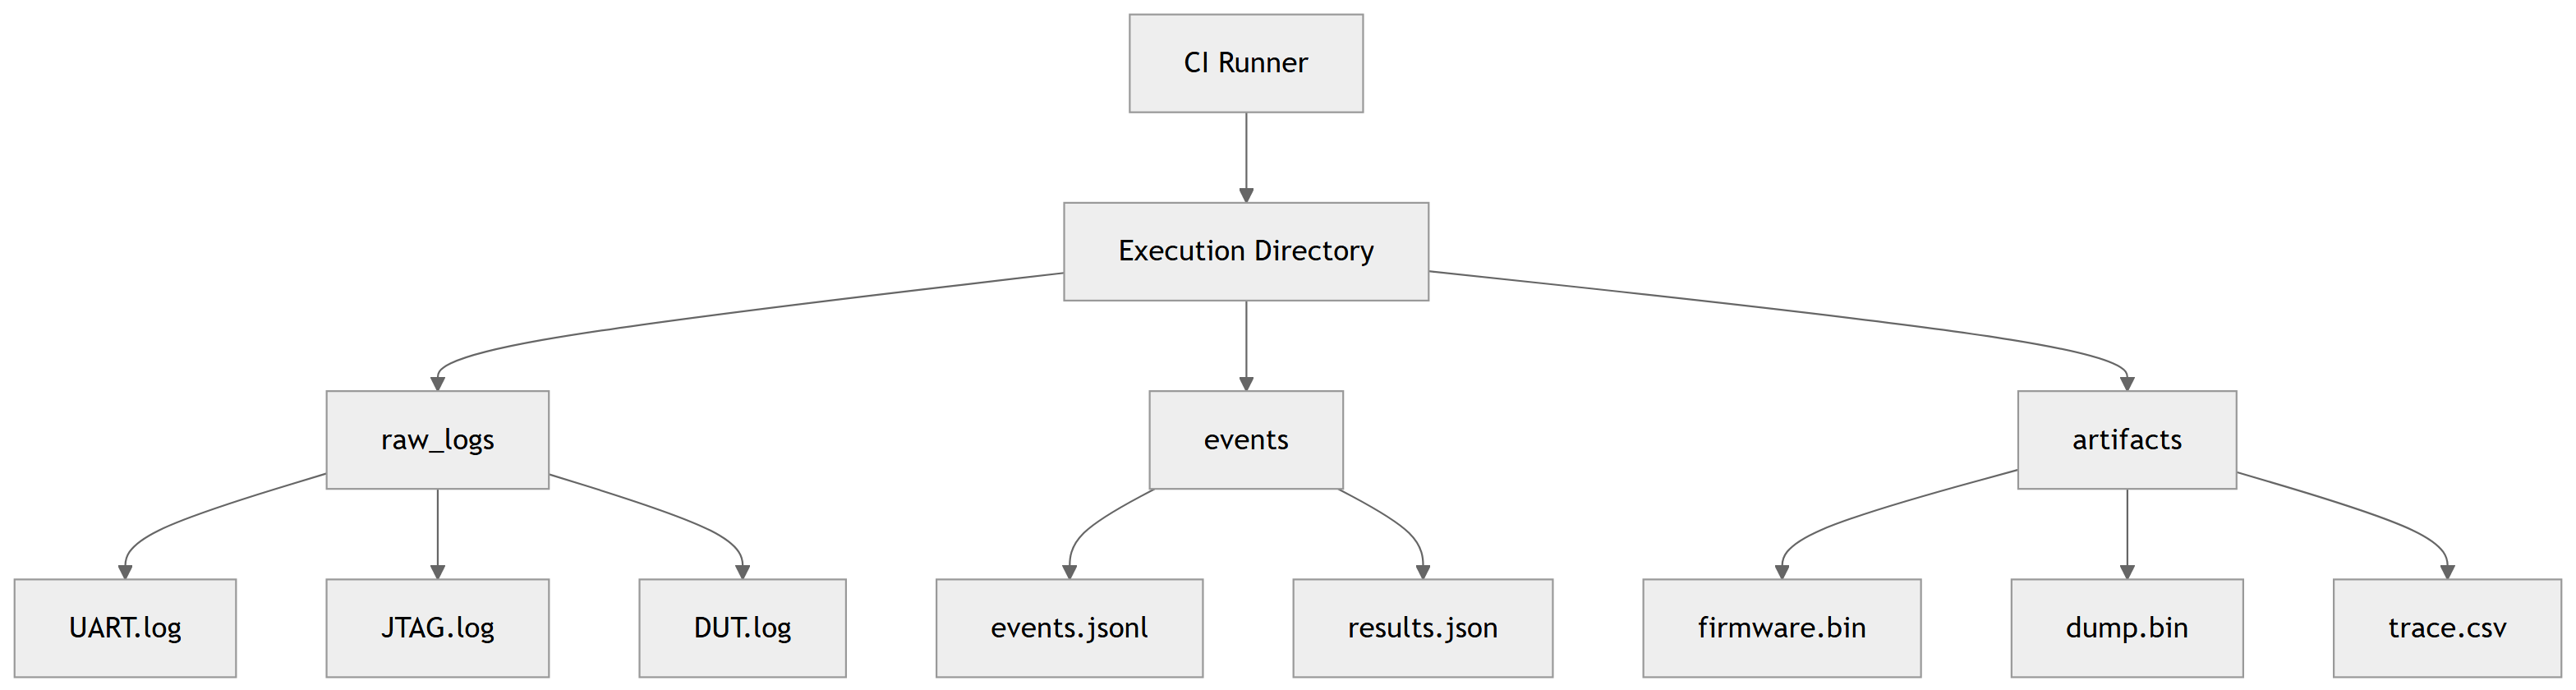
\includegraphics[width=14.82in,height=3.98in]{gtp_logging_v2_files/figure-latex/mermaid-figure-9.png}

}

\caption{\label{fig-storage}Initial CI storage architecture}

\end{figure}%

\subsection{Recommended Execution Directory
Structure}\label{recommended-execution-directory-structure}

\begin{Shaded}
\begin{Highlighting}[]
\NormalTok{EXE{-}20260918{-}001/}
\NormalTok{├── execution.json}
\NormalTok{├── metadata.json}
\NormalTok{├── result.json}
\NormalTok{├── logs/}
\NormalTok{│   ├── framework/framework.log}
\NormalTok{│   ├── dut/uart0.log}
\NormalTok{│   ├── dut/uart1.log}
\NormalTok{│   ├── debug/jtag.log}
\NormalTok{│   └── board/board{-}controller.log}
\NormalTok{├── events/events.jsonl}
\NormalTok{├── measurements/}
\NormalTok{│   ├── power.csv}
\NormalTok{│   ├── temperature.csv}
\NormalTok{│   └── performance.csv}
\NormalTok{├── dumps/}
\NormalTok{│   ├── memory.bin}
\NormalTok{│   └── registers.json}
\NormalTok{├── reports/}
\NormalTok{│   ├── junit.xml}
\NormalTok{│   └── report.html}
\NormalTok{└── artifacts/firmware.bin}
\end{Highlighting}
\end{Shaded}

\subsection{Long-Term Storage}\label{long-term-storage}

\begin{figure}

\centering{

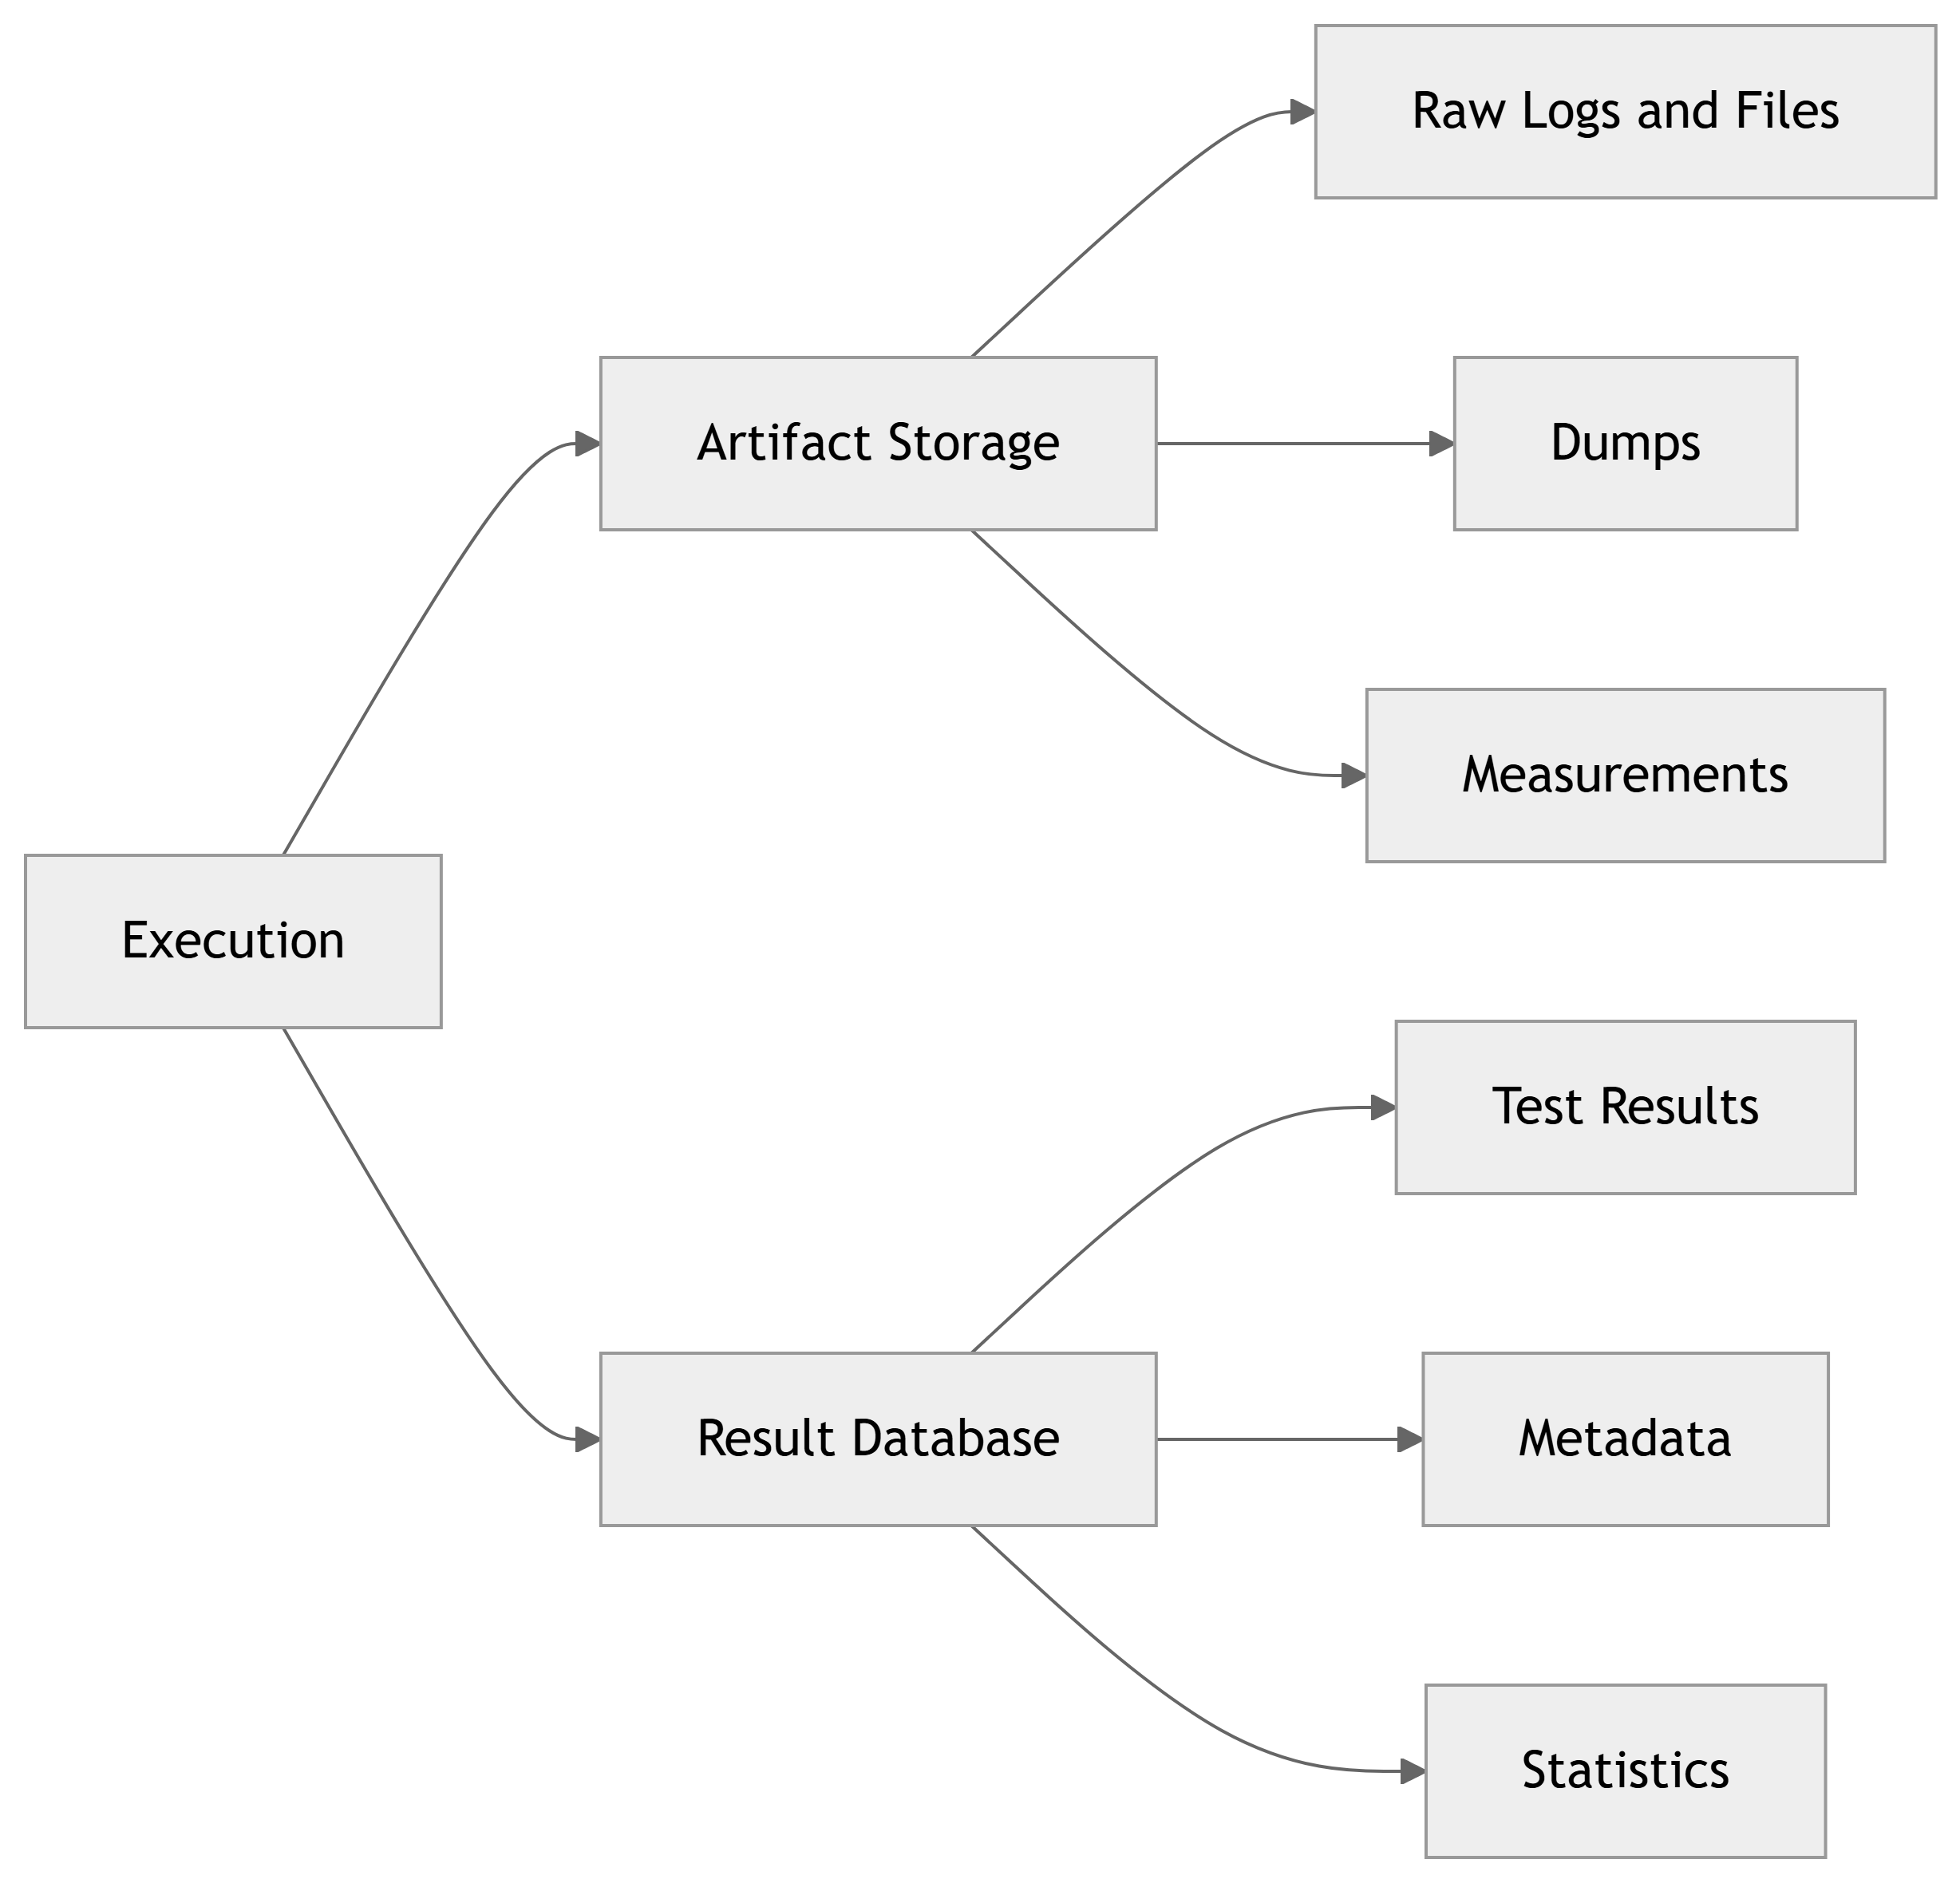
\includegraphics[width=6.4in,height=6.15in]{gtp_logging_v2_files/figure-latex/mermaid-figure-8.png}

}

\caption{\label{fig-long-term-storage}Separation of large artifacts and
searchable metadata}

\end{figure}%

Large raw UART and JTAG logs normally remain in artifact storage rather
than being stored directly in a relational database.

\section{Database Model}\label{database-model}

A simple relational model can be used initially.

\begin{figure}

\centering{

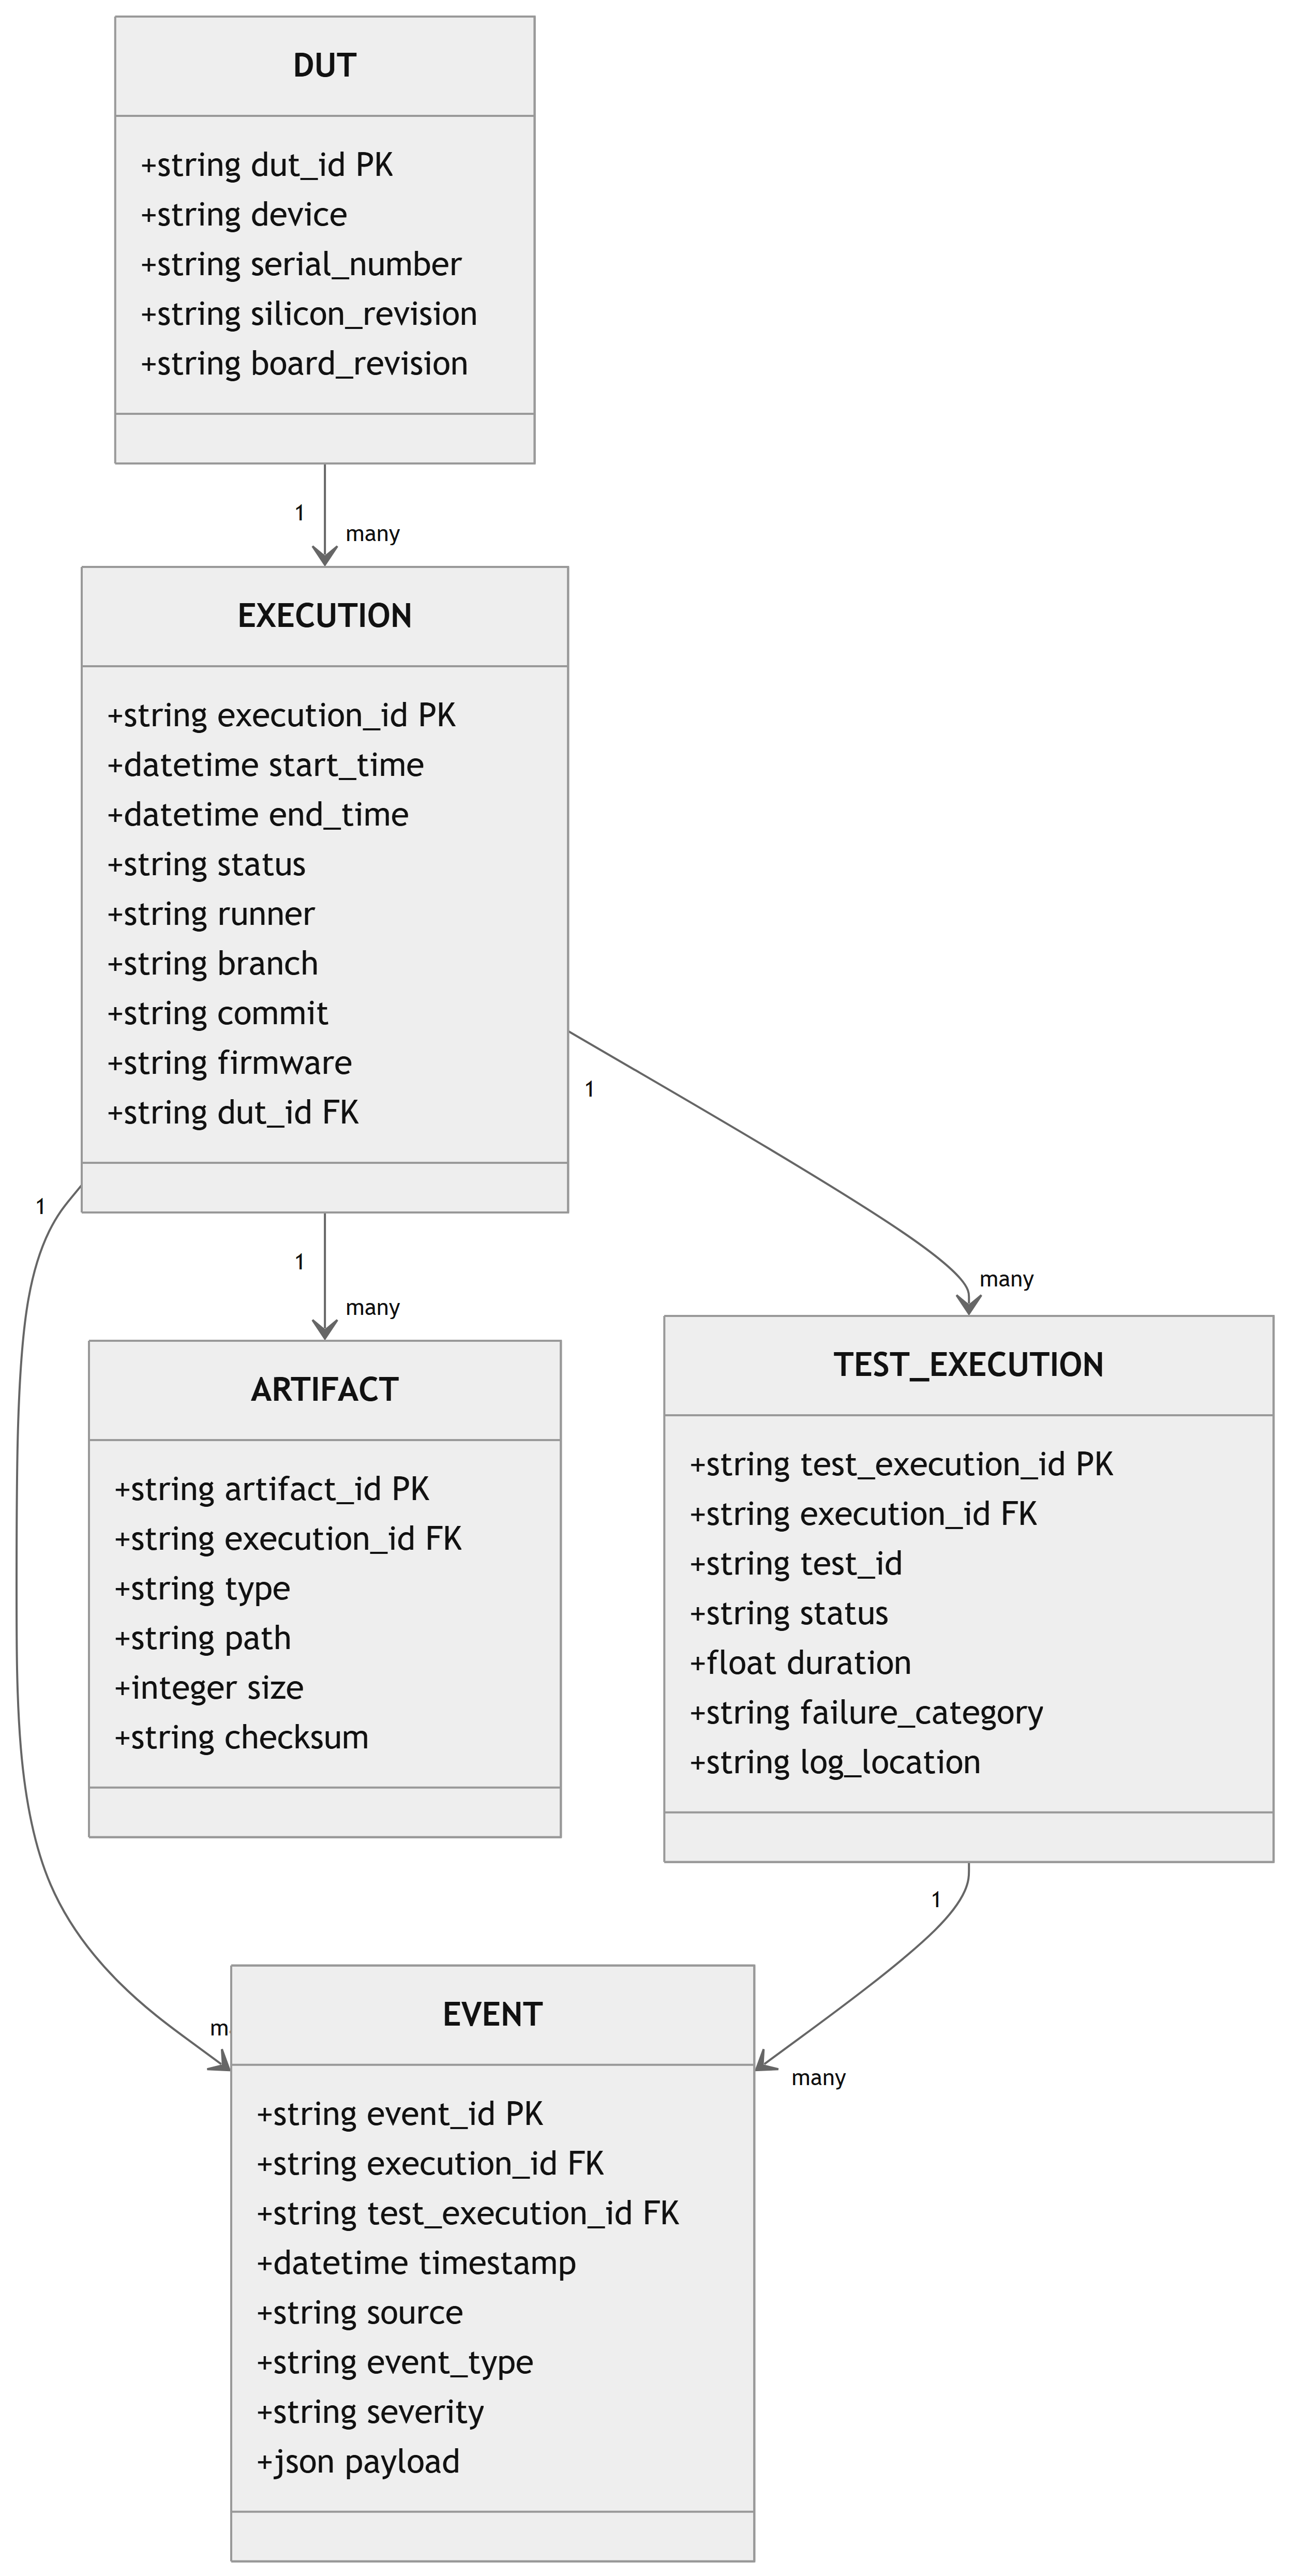
\includegraphics[width=6.5in,height=12.98in]{gtp_logging_v2_files/figure-latex/mermaid-figure-7.png}

}

\caption{\label{fig-database-model}Proposed logging database model}

\end{figure}%

\section{Failure Classification}\label{failure-classification}

Results contain more than a simple PASS or FAIL verdict.

\begin{verbatim}
TEST_FAILURE
ASSERTION_FAILURE
TIMEOUT
UART_FAILURE
JTAG_FAILURE
FLASH_FAILURE
BOOT_FAILURE
DUT_CRASH
DUT_HANG
POWER_FAILURE
COMMUNICATION_FAILURE
INFRASTRUCTURE_FAILURE
ENVIRONMENT_FAILURE
UNKNOWN
\end{verbatim}

\section{Failure Analysis Pipeline}\label{failure-analysis-pipeline}

\begin{figure}

\centering{

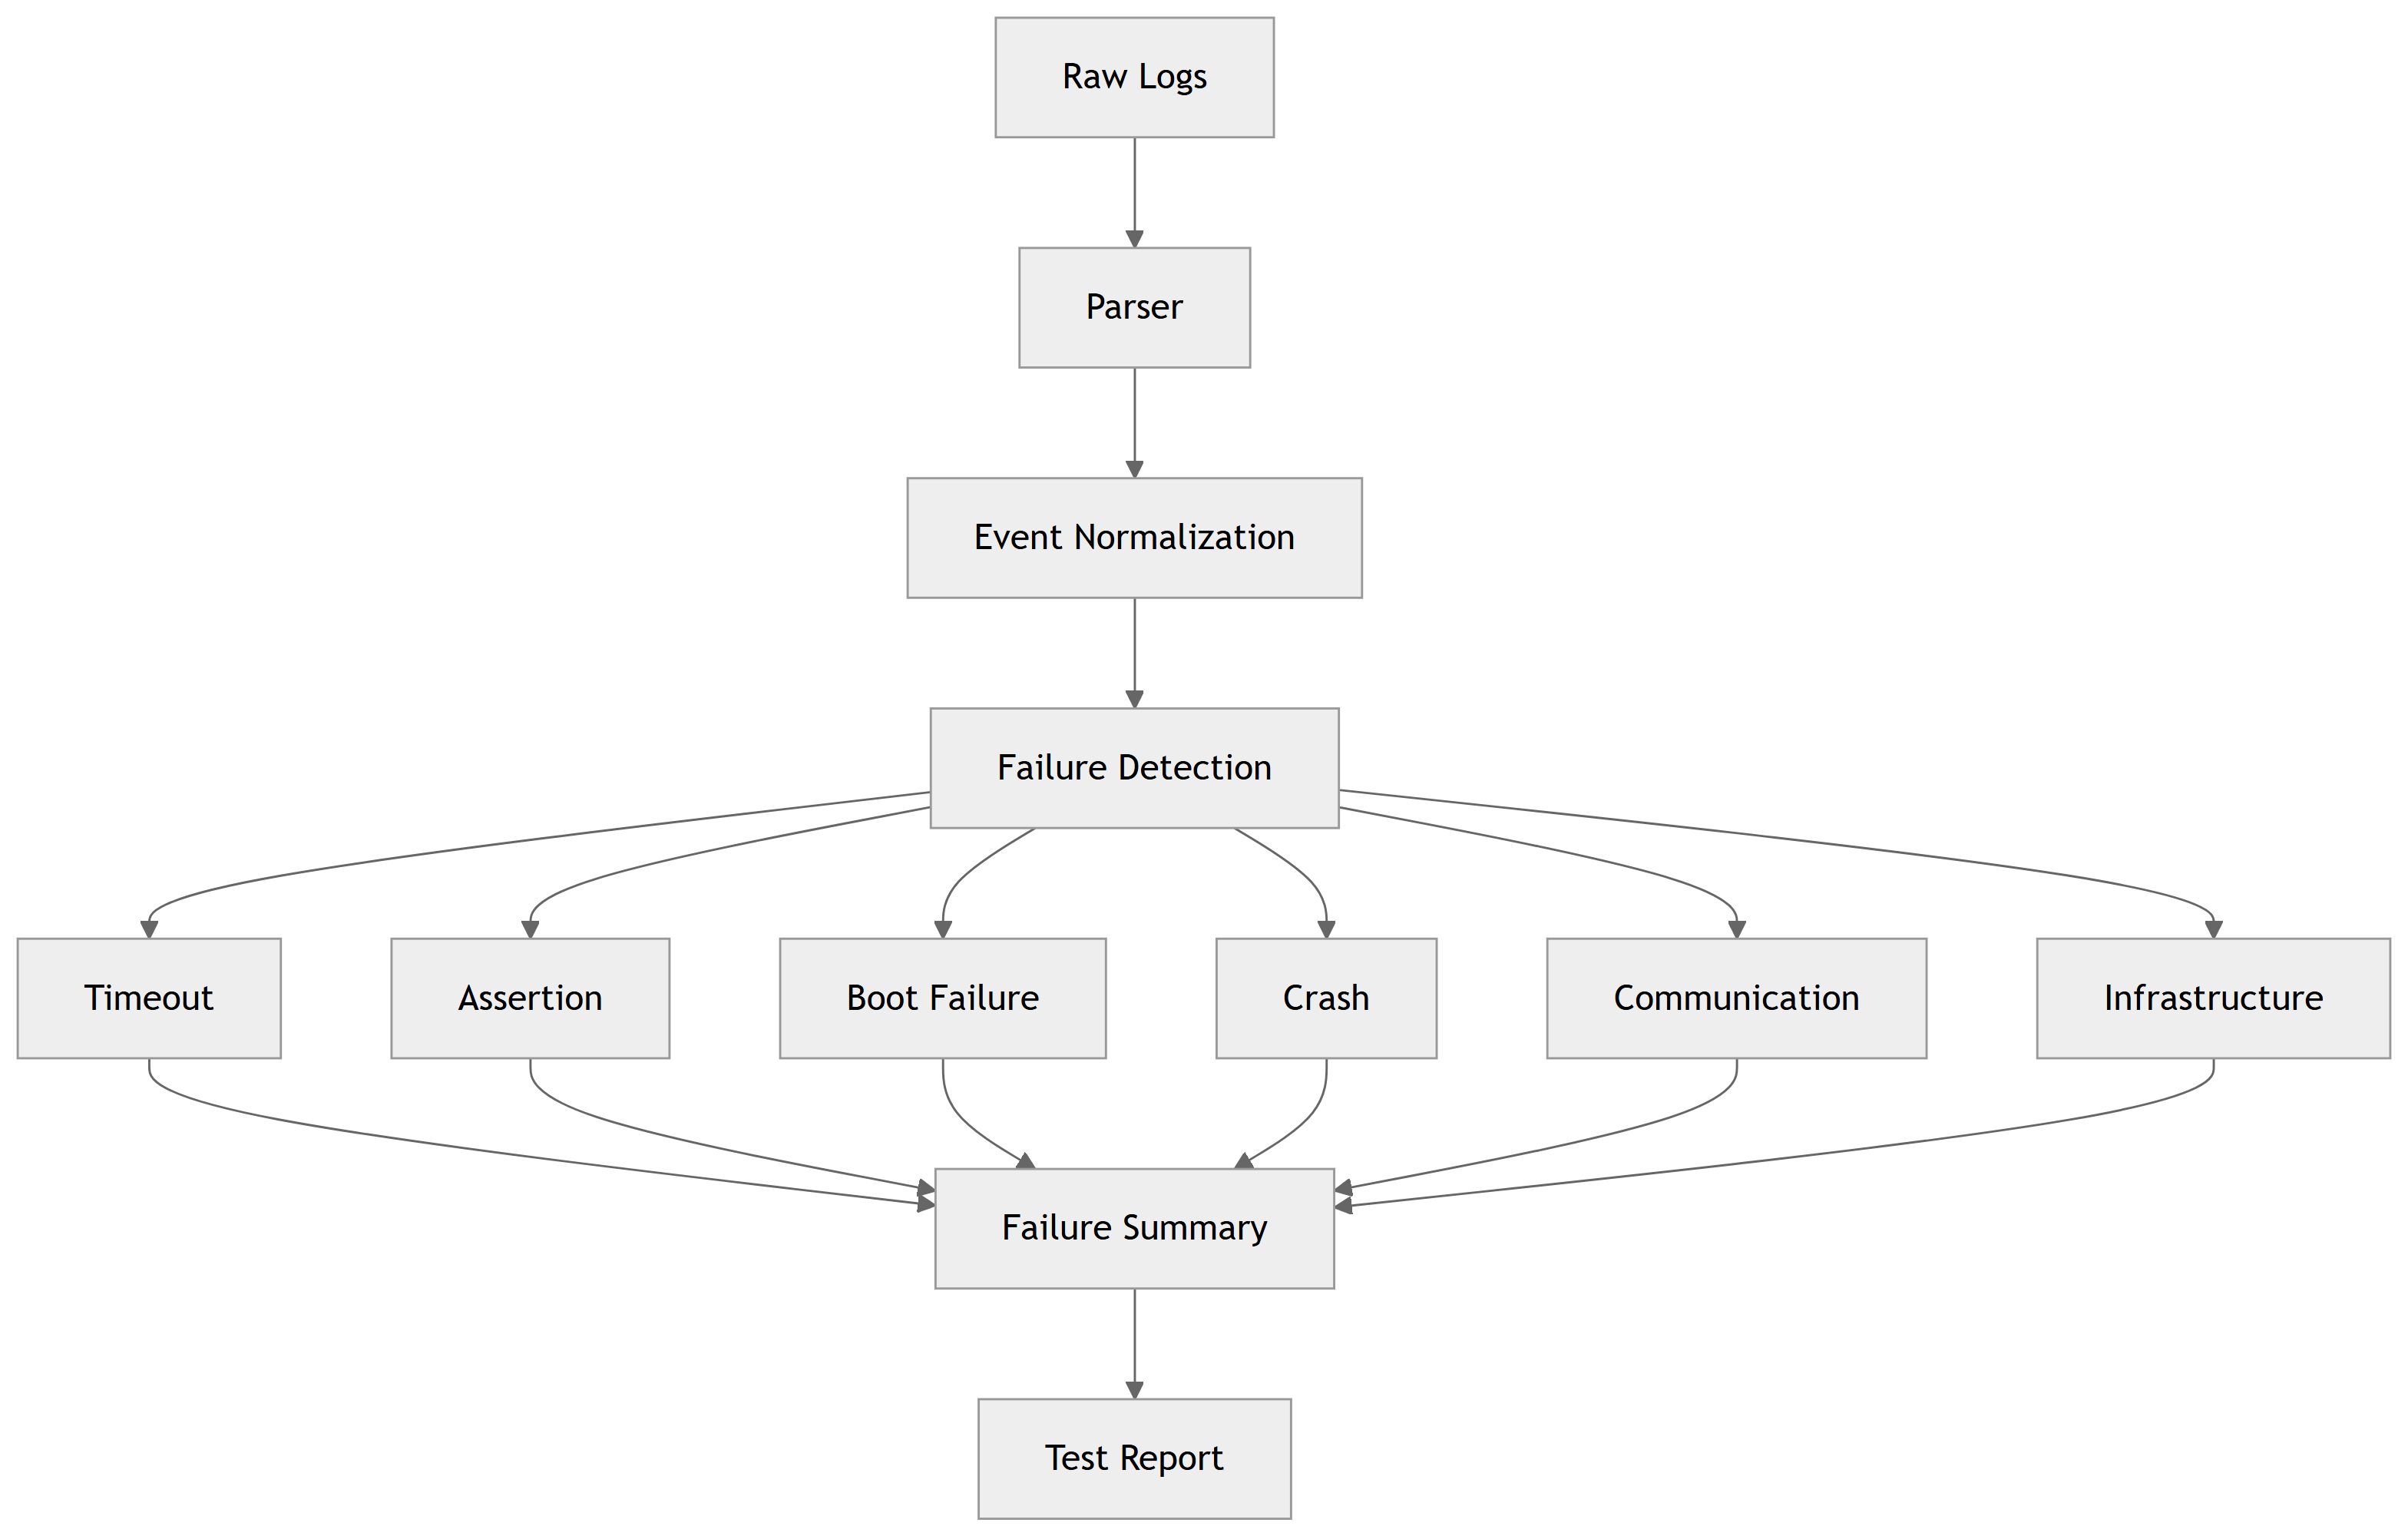
\includegraphics[width=11.33in,height=7.23in]{gtp_logging_v2_files/figure-latex/mermaid-figure-6.png}

}

\caption{\label{fig-failure-analysis}Automated failure-analysis
pipeline}

\end{figure}%

A failure report includes the test identifier, expected and observed
behavior, DUT state, last DUT message, likely failure category, and
links to supporting artifacts.

\section{Test Step Event Example}\label{test-step-event-example}

\begin{Shaded}
\begin{Highlighting}[]
\FunctionTok{\{}
    \DataTypeTok{"timestamp"}\FunctionTok{:} \StringTok{"2026{-}09{-}18T12:31:05.120Z"}\FunctionTok{,}
    \DataTypeTok{"execution\_id"}\FunctionTok{:} \StringTok{"EXE{-}20260918{-}001"}\FunctionTok{,}
    \DataTypeTok{"test\_id"}\FunctionTok{:} \StringTok{"SOC{-}UART{-}001"}\FunctionTok{,}
    \DataTypeTok{"step\_id"}\FunctionTok{:} \StringTok{"STEP{-}005"}\FunctionTok{,}
    \DataTypeTok{"source"}\FunctionTok{:} \StringTok{"test\_framework"}\FunctionTok{,}
    \DataTypeTok{"level"}\FunctionTok{:} \StringTok{"INFO"}\FunctionTok{,}
    \DataTypeTok{"event"}\FunctionTok{:} \StringTok{"STEP\_START"}\FunctionTok{,}
    \DataTypeTok{"message"}\FunctionTok{:} \StringTok{"Send UART command"}
\FunctionTok{\}}
\end{Highlighting}
\end{Shaded}

\section{CI Integration}\label{ci-integration}

\begin{figure}

\centering{

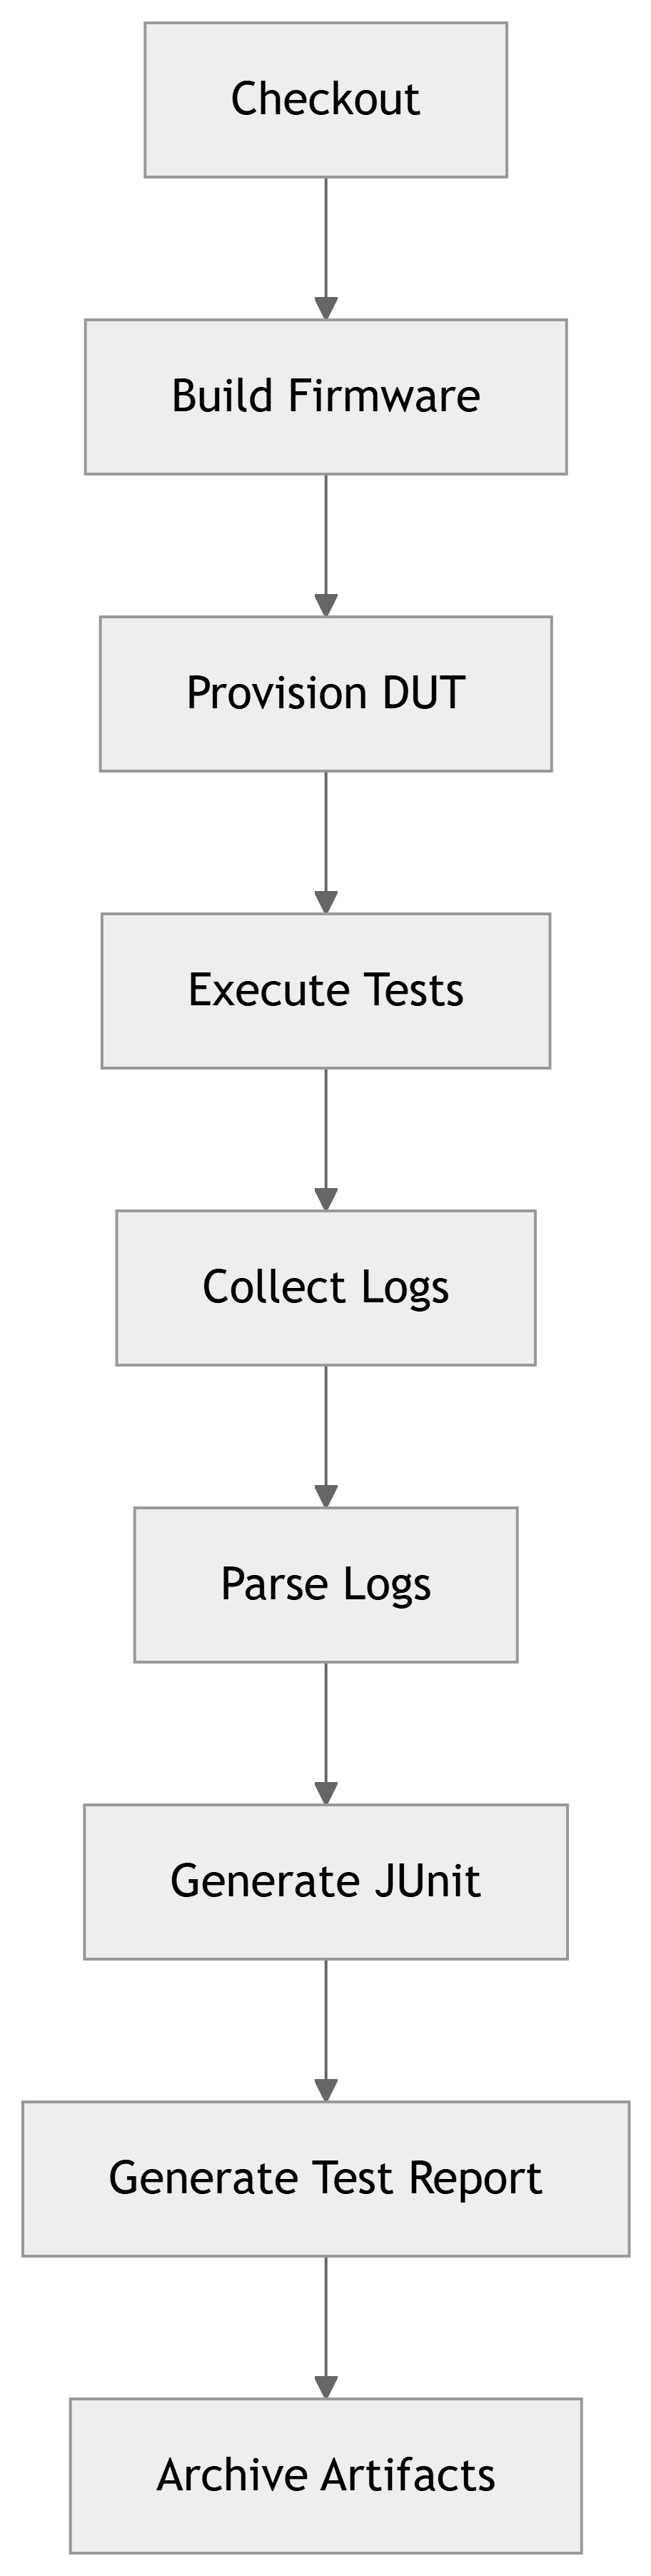
\includegraphics[width=2.38in,height=9.4in]{gtp_logging_v2_files/figure-latex/mermaid-figure-5.png}

}

\caption{\label{fig-ci-pipeline}CI logging and reporting pipeline}

\end{figure}%

JUnit XML is the standard CI test-result interface, while JSONL and raw
logs retain the detailed SoC diagnostic information.

\section{Reporting}\label{reporting}

Execution logging and report generation remain separate concerns.

\begin{figure}

\centering{

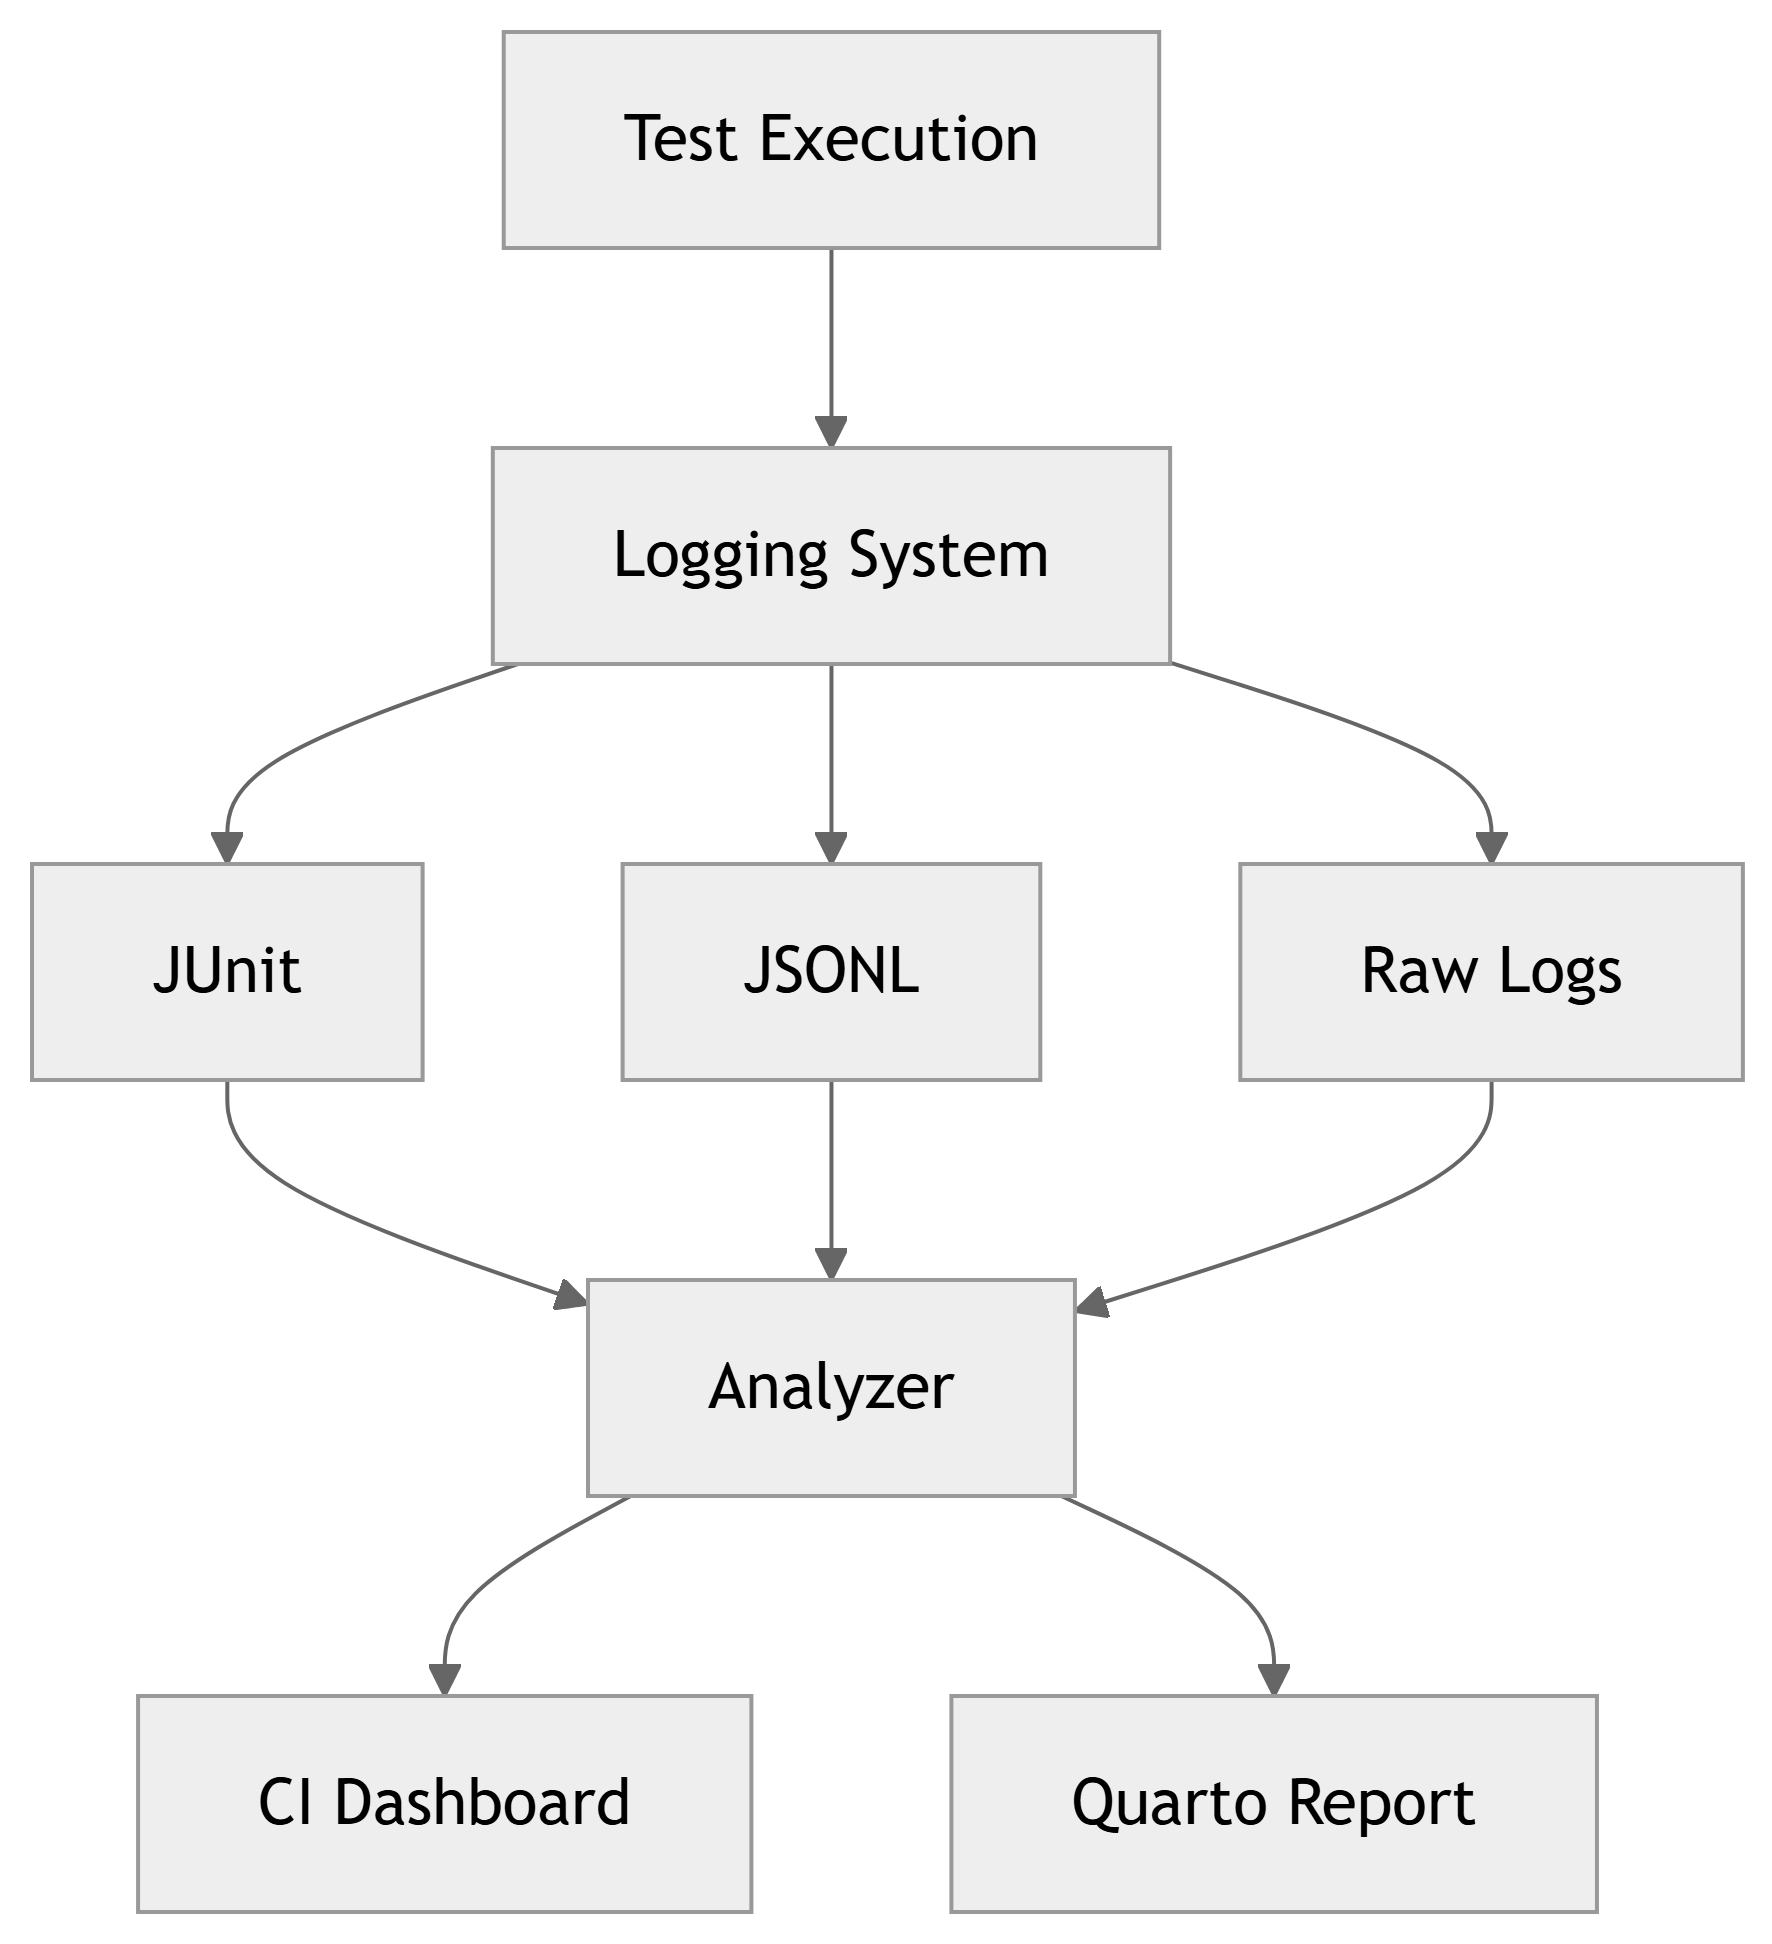
\includegraphics[width=4.62in,height=5.06in]{gtp_logging_v2_files/figure-latex/mermaid-figure-4.png}

}

\caption{\label{fig-reporting}Separation of logging and reporting}

\end{figure}%

Reports support execution summaries, verdict counts, failure categories,
failed-test details, duration, DUT information, firmware and commit
information, and links to raw evidence.

\section{Retention Policy}\label{retention-policy}

Example retention values must be confirmed with the project.

{\def\LTcaptype{none} % do not increment counter
\begin{longtable}[]{@{}ll@{}}
\toprule\noalign{}
Artifact & Example Retention \\
\midrule\noalign{}
\endhead
\bottomrule\noalign{}
\endlastfoot
Test-result metadata & 1 to 2 years \\
Failed-test logs & 1 year \\
Successful raw logs & 30 to 90 days \\
Firmware and build metadata & 1 to 2 years \\
Crash dumps & 1 year \\
Regression reports & 1 to 2 years \\
Debug traces & 30 days \\
\end{longtable}
}

The policy also defines maximum log size, compression, archive format,
deletion policy, ownership, and storage limits.

\section{Log Rotation}\label{log-rotation}

Long-running tests can generate large logs. Rotation can be triggered by
file size, elapsed time, test execution, or DUT reboot.

\begin{verbatim}
uart.log
uart.log.001
uart.log.002
uart.log.003
uart.log.current
\end{verbatim}

Example configurable policy:

\begin{verbatim}
Maximum file size: 100 MB
Compression: gzip
\end{verbatim}

\section{Logging Performance}\label{logging-performance}

Logging must not materially influence the behavior being tested. Use
asynchronous processing, buffering, batching, measurable overhead, and
source-specific controls for high-volume logging.

\begin{verbatim}
LOG_LEVEL=ERROR
\end{verbatim}

may be suitable for a performance-sensitive test, while:

\begin{verbatim}
LOG_LEVEL=TRACE
\end{verbatim}

may be used during debugging.

\section{Security and Sensitive Data}\label{security-and-sensitive-data}

The logging design defines what may be written to logs. Credentials,
tokens, private keys, production secrets, customer information, and
proprietary information require protection or masking.

\begin{verbatim}
username=test_user
password=********
token=********
\end{verbatim}

Sensitive information is not written to raw logs unless explicitly
required and appropriately protected.

\section{Configuration}\label{configuration}

Logging is configurable without modifying test implementation.

\begin{Shaded}
\begin{Highlighting}[]
\FunctionTok{logging}\KeywordTok{:}
\AttributeTok{  }\FunctionTok{level}\KeywordTok{:}\AttributeTok{ INFO}
\AttributeTok{  }\FunctionTok{outputs}\KeywordTok{:}
\AttributeTok{    }\FunctionTok{console}\KeywordTok{:}\AttributeTok{ }\CharTok{true}
\AttributeTok{    }\FunctionTok{file}\KeywordTok{:}\AttributeTok{ }\CharTok{true}
\AttributeTok{    }\FunctionTok{json}\KeywordTok{:}\AttributeTok{ }\CharTok{true}
\AttributeTok{  }\FunctionTok{interfaces}\KeywordTok{:}
\AttributeTok{    }\FunctionTok{uart}\KeywordTok{:}
\AttributeTok{      }\FunctionTok{enabled}\KeywordTok{:}\AttributeTok{ }\CharTok{true}
\AttributeTok{      }\FunctionTok{raw}\KeywordTok{:}\AttributeTok{ }\CharTok{true}
\AttributeTok{    }\FunctionTok{jtag}\KeywordTok{:}
\AttributeTok{      }\FunctionTok{enabled}\KeywordTok{:}\AttributeTok{ }\CharTok{true}
\AttributeTok{  }\FunctionTok{rotation}\KeywordTok{:}
\AttributeTok{    }\FunctionTok{max\_size\_mb}\KeywordTok{:}\AttributeTok{ }\DecValTok{100}
\AttributeTok{    }\FunctionTok{compression}\KeywordTok{:}\AttributeTok{ }\CharTok{true}
\end{Highlighting}
\end{Shaded}

\section{Recommended Initial
Architecture}\label{recommended-initial-architecture}

\begin{figure}

\centering{

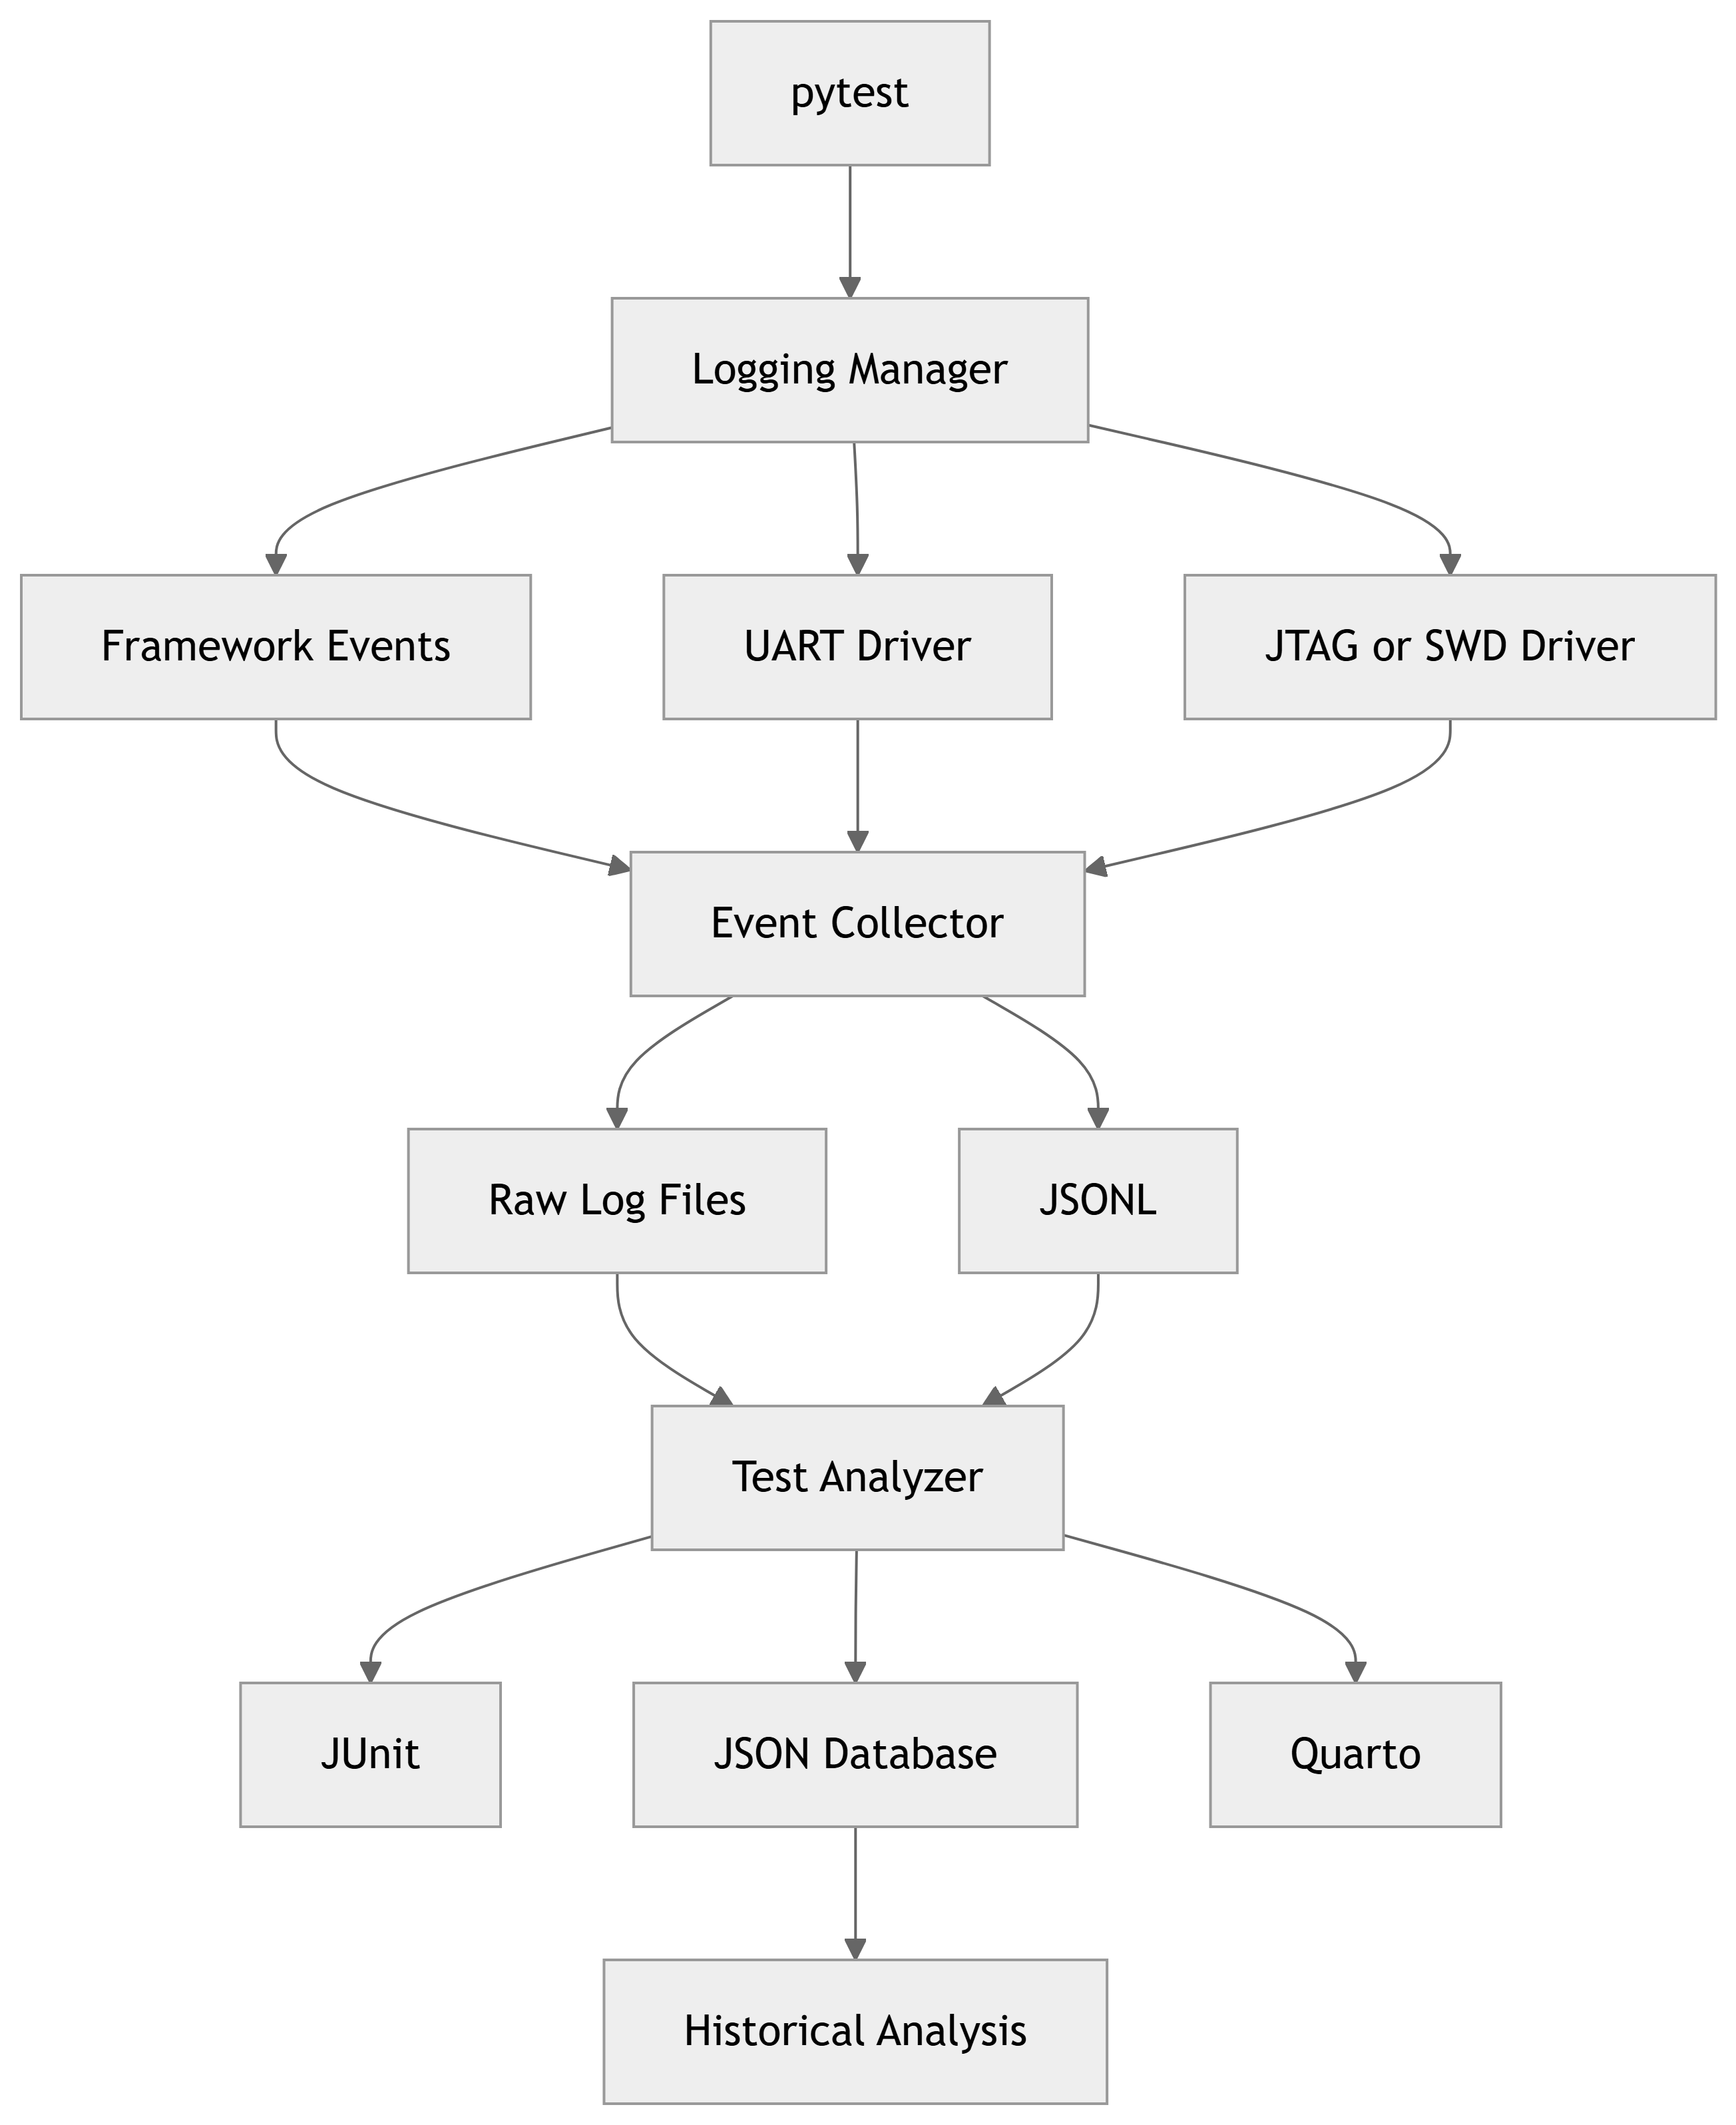
\includegraphics[width=6.8in,height=8.31in]{gtp_logging_v2_files/figure-latex/mermaid-figure-3.png}

}

\caption{\label{fig-initial-architecture}Recommended initial Python and
pytest logging architecture}

\end{figure}%

\section{Recommended Technology
Choices}\label{recommended-technology-choices}

{\def\LTcaptype{none} % do not increment counter
\begin{longtable}[]{@{}ll@{}}
\toprule\noalign{}
Component & Initial Choice \\
\midrule\noalign{}
\endhead
\bottomrule\noalign{}
\endlastfoot
Test framework & pytest \\
Logging API & Python logging plus custom structured logger \\
Canonical event format & JSONL \\
Raw interface logs & Plain text or binary, as appropriate \\
Test result & JUnit XML \\
Metadata & JSON \\
Measurements & CSV or JSON \\
Local storage & Filesystem \\
CI storage & Jenkins or GitLab artifacts \\
Historical data & PostgreSQL or SQLite initially \\
Reporting & Quarto \\
Analysis & Python and pandas \\
Visualization & Quarto and Plotly \\
Compression & gzip or zstd \\
\end{longtable}
}

\section{Key Design Principles}\label{key-design-principles}

\subsection{Preserve Raw Evidence}\label{preserve-raw-evidence}

\textbf{Raw evidence shall never be destroyed as a result of log
processing.} Raw logs remain available after parsing and analysis.

\subsection{Every Event Must Be
Traceable}\label{every-event-must-be-traceable}

\begin{figure}

\centering{

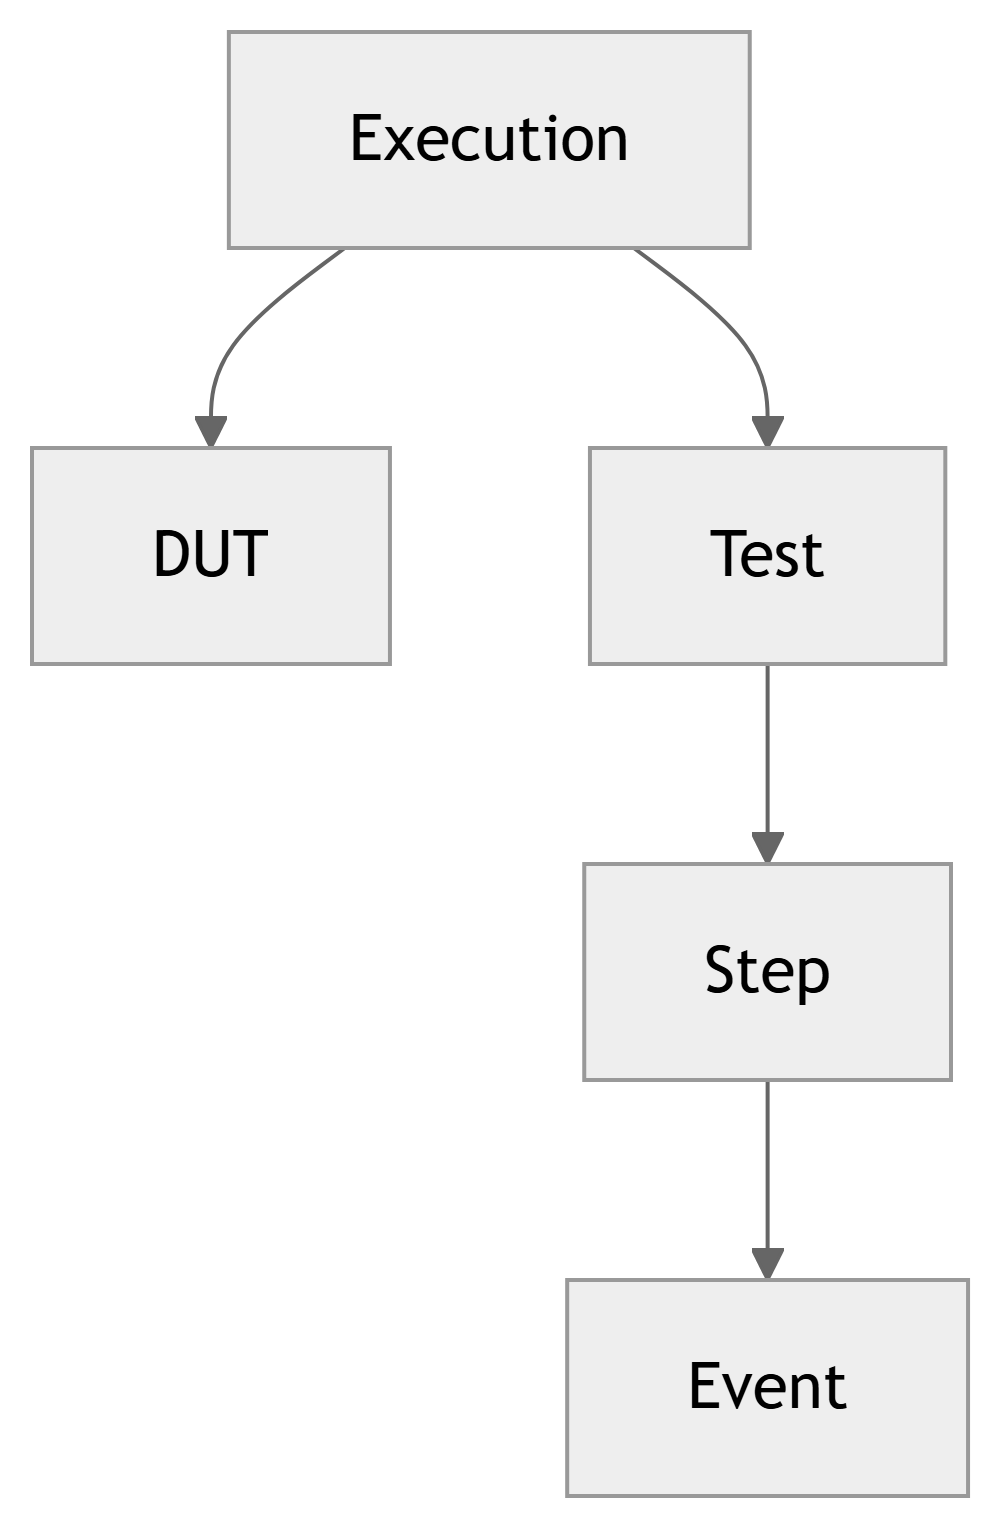
\includegraphics[width=2.6in,height=3.98in]{gtp_logging_v2_files/figure-latex/mermaid-figure-2.png}

}

\caption{\label{fig-traceability}Required event traceability hierarchy}

\end{figure}%

\subsection{Test Results and Logs Are
Different}\label{test-results-and-logs-are-different}

A test result answers: \textbf{Did the test pass or fail?}

A log answers: \textbf{What happened during execution?}

The two are linked but are not the same data product.

\subsection{Logs Must Support Failure
Reconstruction}\label{logs-must-support-failure-reconstruction}

The stored information must allow failure reconstruction without access
to the original test-runner session.

\subsection{Logging Must Be
Configurable}\label{logging-must-be-configurable}

At minimum, support \texttt{ERROR}, \texttt{WARNING}, \texttt{INFO},
\texttt{DEBUG}, and \texttt{TRACE}, together with source-specific
configuration.

\subsection{Logging Must Be Low
Overhead}\label{logging-must-be-low-overhead}

Logging must not materially alter timing-sensitive,
performance-sensitive, or power-sensitive SoC validation behavior.

\section{Final Architectural
Principle}\label{final-architectural-principle}

\begin{quote}
\textbf{A test execution log shall contain sufficient information to
reconstruct and diagnose the execution without requiring access to the
original test-runner session.}
\end{quote}

The supporting principle is:

\begin{quote}
\textbf{Raw evidence shall be preserved independently from processed and
analyzed results.}
\end{quote}

Together, these principles drive event structure, correlation
identifiers, storage, retention, analysis, and reporting.

\section{Rendering}\label{rendering}

Place \texttt{my\_template.docx} in the same directory as this
\texttt{.qmd} file, then render all configured formats:

\begin{verbatim}
quarto render test_execution_logging.qmd
\end{verbatim}

Quarto creates HTML, DOCX, and PDF outputs. PDF output requires a
supported TeX installation. Mermaid diagrams are authored as Quarto
Mermaid cells and are rendered rather than shown as raw diagram text.




\end{document}
